\documentclass[a4paper,11pt]{article}
\usepackage[UKenglish]{babel}
\usepackage[table]{xcolor}
\usepackage{graphicx}
\usepackage{courier}
\usepackage{color}
\usepackage{array}
\usepackage{pstricks}
\usepackage{parskip}
\usepackage[bottom]{footmisc}
\usepackage{fancyhdr}
\usepackage{multirow}
\usepackage{longtable}
\usepackage{listings}
\usepackage{siunitx}
% the hyperref package must always be the last package to be included
\usepackage[pdftex,
            pdfusetitle,
            pdfsubject={Programmer's Reference Guide for dastaZ80 homebrew computer},
            pdfkeywords={Z80, homebrew computer, Operating System, OS, programmer, reference, guide}
        ]{hyperref}

\hypersetup{
    colorlinks = true,
    linkcolor = blue,
    anchorcolor = blue,
    citecolor = blue,
    filecolor = blue,
    urlcolor = blue
}

\setlength\parindent{0pt}

\begin{document}
    \pagestyle{empty}
    % ==========================================================================
    % Cover page
    % ==========================================================================
    \begin{pspicture}(8.5,11)
        \rput[b](3.5,8){
            \parbox{7in}{
                \begin{flushright}
                    \Huge\bfseries\sffamily dastaZ80 Mark II\\ Programmer's Reference Guide
                \end{flushright}
            }
        }
        \uput[0](0,0){\color{blue}\rule{7in}{0.5ex}}
    \end{pspicture}
    \title{dastaZ80 Programmer's Reference Guide}
    \author{David Asta}
    \date{1 October 2022}

    \pagebreak
    % ==========================================================================
    % Header & Footer
    % ==========================================================================
    \pagestyle{fancy}
    \fancyhf{}
    \fancyhead[R]{dastaZ80 Mark II Programmer's Reference Guide}
    % ==========================================================================
    \section*{Disclaimer}
    % ==========================================================================
    The products described in this manual are intended for educational purposes,
    and should not be used for controlling any machinery, critical component in
    life support devices or any system in which failure could result in personal
    injury if any of the described here products fail.
    
    These products are subject to continuous development and improvement. All
    information of a technical nature and particulars of the products and its
    use are given by the author in good faith. However, it is acknowledged that
    there may be errors or omissions in this manual. Therefore, the author
    cannot accept any liability for any loss or damage arising from the use of
    any information or particulars in this manual.

    % ==========================================================================
    \section*{Licenses}
    % ==========================================================================
    \small
    \textbf{Hardware} is licensed under the \textbf{Creative Commons
    Attribution-ShareAlike 4.0 International License}
    
    \hspace{1cm}http://creativecommons.org/licenses/by-sa/4.0/
    
    \textbf{Software} is licensed under \textbf{The MIT License}
    
    \hspace{1cm}https://opensource.org/licenses/MIT
    
    \textbf{Documentation} is licensed under the \textbf{Creative Commons
    Attribution-ShareAlike 4.0 International License}
    
    \hspace{1cm}http://creativecommons.org/licenses/by-sa/4.0/

    \normalsize

    \hrulefill

    \textcopyright 2023 David Asta

    \pagebreak
    % ==========================================================================
    \section*{Document Conventions}
    % ==========================================================================
    The following conventions are used in this manual:

    \begin{center}
        \begin{tabular}{c m{9cm}}
            \hline
            MUST & MUST denotes that the definition is and absolute
            requirement.\\
            \hline
            SHOULD & SHOULD denotes that it is recommended, but that there may
            exist valid reasons to ignore it.\\
            \hline
            \textbf{DEVICE} & Device names are displayed in bold all upper case 
            letters, and refer to hardware devices.\\
            \hline
            \texttt{Courier} & Text appearing in the \texttt{Courier} font 
            represents either an OS System Variable a Z80 CPU Register
            or a Z80 Flag. OS System Variables are identifiers for specific
            \textbf{MEMORY} addresses that can be used to read statuses and to
            pass information between routines or programs.\\
            \hline
            \texttt{0x14B0} & Numbers prefixed by 0x indicate an Hexadecimal value.
            Unless specified, memory addresses are always expressed in
            Hexadecimal.\\
            \hline
            F\_abcdef & Text starting with F\_ refers to the name of an OS 
            routine that can be called via Jumpblocks. \\
            \hline
            \textit{jp} abcdef & Refers to the Z80 mnemonic for \textit{jump},
            which transfers the CPU Program Counter to a specific \textbf{MEMORY}
            address.\\
            \hline
        \end{tabular}
    \end{center}

    The SD card is referred as \textbf{DISK}.
    
    The Floppy Disk Drive is referred as \textbf{DISK} or as \textbf{FDD}.

    The 80 column text VGA output is referred as \textbf{CONSOLE} or as
    \textbf{High Resolution Display}.

    The 40 column graphics Composite Video output is referred as \textbf{Low
    Resolution Display} or \textbf{VDP screen}.

    The Operating System may be referred as DZOS, dzOS or simply OS.

    \textbf{MEMORY} refers to both \textbf{ROM} and \textbf{RAM}.

    Memory used by the \textbf{Low Resolution Display} is referred as
    \textbf{VRAM} (Video RAM).

    In the list of routines, the \textbf{Destroys} lists the \textbf{CPU}
    registers and \textbf{MEMORY} System Variables that are destroyed by the
    routine in question. But bare in mind that a routine may call other routines
    that may destroy other registers and variables. Refer to the \textbf{Calls}
    list to check the entire flow. By \textit{Destroys} is understood that the
    listed register or variable value is overwritten within the routine.

    \pagebreak
    % ==========================================================================
    \section*{Related Documentation}
    % ==========================================================================
    \begin{itemize}
        \item dastaZ80 User's Manual\cite{dastaz80userman}
        \item dastaZ80 Technical Reference Manual\cite{dastaz80techman}
        \item dzOS Github Repository\cite{dastaZ80github}
    \end{itemize}

    \pagebreak
    % ==========================================================================
    \tableofcontents
    % ==========================================================================

    \pagebreak
    % ==========================================================================
    % Header & Footer
    % ==========================================================================
    \pagestyle{fancy}
    \fancyhf{}
    \fancyhead[R]{dastaZ80 Mark II Programmer's Reference Guide}
    \fancyfoot[R]{\thepage}
    \setcounter{page}{1}
    % ==========================================================================
    \section{Memory Map}
    % ==========================================================================
    
    % ==========================================================================
    \subsection{ROM}
    % ==========================================================================

    The \textbf{ROM} is a 16KB EEPROM, and is divided as follows:

    \begin{tabular}{ |m{1.3cm}|m{1.3cm}|m{3.3cm}|m{2.7cm}|>{\raggedleft\arraybackslash}m{2cm}| }
        \hline
        \rowcolor{lightgray}
        \multicolumn{2}{|c|}{Address} &
        \multicolumn{2}{|c|}{Description} &
        Size (bytes) \\
        \hline
        \hline
        \texttt{0x0000} & \texttt{0x0007} & Cold Boot & \textbf{\multirow{3}{4em}{BIOS}} & 8 \\
        \texttt{0x0008} & \texttt{0x0215} & init SIO/2 & & 526 \\
        \texttt{0x0216} & \texttt{0x133F} & BIOS code & & 4,394 \\
        \hline
        \texttt{0x1340} & \texttt{0x26C7} & Kernel code & \textbf{\multirow{2}{4em}{Kernel}} & 5,000 \\
        \texttt{0x26B7} & \texttt{0x26C7} & dzOS version build & & 17 \\
        \hline
        \texttt{0x26C8} & \texttt{0x3A88} & CLI code & \textbf{CLI} & 5,057 \\
        \hline
        \texttt{0x3A89} & \texttt{0x3AB6} & Bootstrap & \textbf{BOOTSTRAP} & 46 \\
        \hline
        \texttt{0x3AB7} & \texttt{0x3E0E} & VDP dastaZ80 Logo & & 856 \\
        \hline
        \texttt{0x3E4A} & \texttt{0x3EFD} & BIOS Jumpblock & \textbf{\multirow{2}{4em}{Jumpblocks}} & 180 \\
        \texttt{0x3EFE} & \texttt{0x3FFF} & Kernel Jumpblock & & 258 \\
        \hline
    \end{tabular}

    % ==========================================================================
    \subsection{RAM}
    % ==========================================================================

    The \textbf{RAM} is a 64KB SRAM, and is divided as follows:

    \begin{longtable}{ |l|l|l|l|l| }\hline
        \hline
        \rowcolor{lightgray}
        \multicolumn{2}{|c|}{Address} &
        \multicolumn{2}{|c|}{Description} &
        Size (bytes) \\
        \hline
        \hline
        \endfirsthead

        \hline
        \rowcolor{lightgray}
        \multicolumn{2}{|c|}{Address} &
        \multicolumn{2}{|c|}{Description} &
        Size (bytes) \\
        \hline
        \hline
        \endhead

        \texttt{0x4000} & \texttt{0x401F} 
        & \multicolumn{2}{|l|}{\textbf{Stack}} & 32\\
        \hline
        \texttt{0x4020} & \texttt{0x4174} 
        & \multicolumn{2}{|l|}{\textbf{System Variables}} & 373\\
        \hline
        \texttt{0x4188} & \texttt{0x421F} 
        & \multicolumn{2}{|l|}{\textbf{Reserved for future use}} & 139\\
        \hline
        \texttt{0x4220} & \texttt{0x441F} 
        & \multicolumn{2}{|l|}{\textbf{DISK Buffer}} & 512\\
        \hline
        \texttt{0x4420} & \texttt{0xFFFF} 
        & \multicolumn{2}{|l|}{\textbf{Free RAM}} & 48,096\\
        \hline
      \end{longtable}

    % ==========================================================================
    \subsubsection{Stack}
    % ==========================================================================

    A \textit{Stack} is a list of words (2 bytes) that uses Last In First Out 
    (LIFO) access method. It is used by the \textbf{CPU} to keep track of
    \textbf{MEMORY} addresses when executing a \textit{call} instruction.

    The programmer can also store (\textit{PUSH}) or retrieve (\textit{POP})
    values on/from the top of the stack.

    Usage of the Stack requires very careful attention. doing (\textit{PUSH})
    without the corresponding (\textit{POP}) or vice versa, will set the CPU on
    the wrong path of execution. Most of the time just hanging the computer, but
    also potentially destroying information if an access to disk is triggered by
    the wrong call.

    % ==========================================================================
    \subsubsection{System Variables (SYSVARS)}
    % ==========================================================================
    \label{sec:ram_memmap}

    The area of \textbf{RAM} called \textit{System Variables (SYSVARS)} is an 
    area heavily used by the OS, but it can also be used by a program to
    communicate with the OS.

    The area has been \textit{split} as follows:

    \begin{itemize}
        \item \textbf{SIO}
        \begin{itemize}
            \item \texttt{0x4020} - \textbf{SIO\_CH\_A\_BUFFER} (64 bytes):
            Buffer for SIO Channel A.
            \item \texttt{0x4060} - \textbf{SIO\_CH\_A\_IN\_PTR} (2 bytes)
            \item \texttt{0x4062} - \textbf{SIO\_CH\_A\_RD\_PTR} (2 bytes)
            \item \texttt{0x4064} - \textbf{SIO\_CH\_A\_BUFFER\_USED} (1 byte)
            \item \texttt{0x4065} - \textbf{SIO\_CH\_A\_LASTCHAR} (1 bytes)
            \item \texttt{0x4066} - \textbf{SIO\_CH\_B\_BUFFER} (64 bytes):
            Buffer for SIO Channel B.
            \item \texttt{0x40A6} - \textbf{SIO\_CH\_B\_IN\_PTR} (2 bytes)
            \item \texttt{0x40A6} - \textbf{SIO\_CH\_B\_RD\_PTR} (2 bytes)
            \item \texttt{0x40AA} - \textbf{SIO\_CH\_B\_BUFFER\_USED} (1 byte)
        \end{itemize}
        \item \textbf{DISK Superblock}
        \begin{itemize}
            \item \texttt{0x40AB} - \textbf{DISK\_is\_formatted} (1 byte): tells
            to the OS if the \textbf{DISK} can be used.
            \begin{itemize}
                \item \texttt{0xFF} = formatted with \textit{DZFS}.
                \item \texttt{0x00} = not formatted.
            \end{itemize}
            \item \texttt{0x40AC} - \textbf{DISK\_show\_deleted} (1 byte)
            \begin{itemize}
                \item \texttt{0x00} = do not show deleted files in \textit{cat}
                command results.
                \item \texttt{0x01} = show also deleted files in \textit{cat}
                command results.
            \end{itemize}
            \item \texttt{0x40AD} - \textbf{DISK\_cur\_sector} (2 bytes): current
            Sector being used by the OS.
        \end{itemize}
        \item \textbf{DISK BAT}
        \begin{itemize}
            \item \texttt{0x40AF} - \textbf{DISK\_cur\_file\_name} (14 bytes): 
            Filename of file currently being load or saved.
            \item \texttt{0x40BD} - \textbf{DISK\_cur\_file\_attribs} (1 byte):
            Attributes of file currently being load or saved.
            \begin{itemize}
                \item Bit 0: if set, file is Read Only.
                \item Bit 1: if set, file is Hidden (it does not display in
                \textit{cat} command results).
                \item Bit 2: if set, file is System (it does not display in
                \textit{cat} command results).
                \item Bit 3: if set, file is Executable.
                \item Bits 4-7: not used.
            \end{itemize}
            \item \texttt{0x40BE} - \textbf{DISK\_cur\_file\_time\_created} (2
            bytes): time when currently being load or saved file was created.
            \item \texttt{0x40C0} - \textbf{DISK\_cur\_file\_date\_created} (2
            bytes): date when currently being load or saved file was created.
            \item \texttt{0x40C2} - \textbf{DISK\_cur\_file\_time\_modified} (2
            bytes): time when currently being load or saved file was last modified.
            \item \texttt{0x40C4} - \textbf{DISK\_cur\_file\_date\_modified} (2
            bytes): date when currently being load or saved file was last modified.
            \item \texttt{0x40C6} - \textbf{DISK\_cur\_file\_size\_bytes} (2
            bytes): size in bytes of file currently being load or saved.
            \item \texttt{0x40C8} - \textbf{DISK\_cur\_file\_size\_sectors} (1
            byte): size in sectors of file currently being load or saved.
            \item \texttt{0x40C9} - \textbf{DISK\_cur\_file\_entry\_number} (2
            bytes): entry number in the BAT, of file currently being load or
            saved.
            \item \texttt{0x40CB} - \textbf{DISK\_cur\_file\_1st\_sector} (2
            bytes): sector number, of the first sector, where the bytes of file
            currently being load or saved are stored in the \textbf{DISK}.
            \item \texttt{0x40CD} - \textbf{DISK\_cur\_file\_load\_addr} (2
            bytes): address where the bytes of file currently being load will be
            stored in \textbf{RAM}.
        \end{itemize}
        \item \textbf{CLI}: buffers used by CLI to store temporary data.
        \begin{itemize}
            \item \texttt{0x40CF} - \textbf{CLI\_prompt\_addr} (2 bytes): The
            address of the CLI Prompt subroutine. Programs that need to return
            control to CLI on exit, MUST jump to the address stored here.
            \item \texttt{0x40D1} - \textbf{CLI\_buffer} (6 bytes): generic
            buffer.
            \item \texttt{0x40D7} - \textbf{CLI\_buffer\_cmd} (16 bytes): when a
            user enters a command and its parameters, the command alone is
            stored here.
            \item \texttt{0x40E7} - \textbf{CLI\_buffer\_parm1\_val} (16 bytes):
            when a user enters a command and its parameters, the first parameter
            is stored here.
            \item \texttt{0x40F7} - \textbf{CLI\_buffer\_parm2\_val} (16 bytes):
            when a user enters a command and its parameters, the second parameter
            is stored here.
            \item \texttt{0x4107} - \textbf{CLI\_buffer\_pgm} (32 bytes): generic
            buffer.
            \item \texttt{0x4127} - \textbf{CLI\_buffer\_full\_cmd} (64 bytes):
            when a user enters a command and its parameters, the entire line
            entered by the user is stored here. This is useful for passing
            parameters to programs called with \textit{run} command.
        \end{itemize}
        \item \textbf{RTC}
        \begin{itemize}
            \item \texttt{0x4167} - \textbf{RTC\_hour} (1 byte): 24h format,
            in hexadecimal (\texttt{0x00}-\texttt{0x17}).
            \item \texttt{0x4168} - \textbf{RTC\_minutes} (1 byte): in
            hexadecimal (\texttt{0x00}-\texttt{0x3B}).
            \item \texttt{0x4169} - \textbf{RTC\_seconds} (1 byte): in
            hexadecimal (\texttt{0x00}-\texttt{0x3B}).
            \item \texttt{0x416A} - \textbf{RTC\_century} (1 byte): 20 part of
            year 20xx, in hexadecimal (\texttt{0x14} = 20).
            \item \texttt{0x416B} - \textbf{RTC\_year} (1 byte): xx part of
            year 20xx, in hexadecimal (e.g. \texttt{0x16} = 22). The \textbf{RTC}
            supports until 2079, therefore maximum value is \texttt{0x4F}.
            \item \texttt{0x416C} - \textbf{RTC\_year4} (2 bytes): four digit
            year, in hexadecimal (e.g. \texttt{0x07E6} = 2022). The \textbf{RTC}
            supports until 2079, therefore maximum value is \texttt{0x081F}.
            \item \texttt{0x416E} - \textbf{RTC\_month} (1 byte): in
            hexadecimal (\texttt{0x00}-\texttt{0x0C}).
            \item \texttt{0x416F} - \textbf{RTC\_day} (1 byte): in hexadecimal
            (\texttt{0x00}-\texttt{0x1F}).
            \item \texttt{0x4170} - \textbf{RTC\_day\_of\_the\_week} (1 byte):
            \texttt{0x00}=Sunday, \texttt{0x01}=Monday, \texttt{0x02}=Tuesday,
            \texttt{0x03}=Wednesday, \texttt{0x04}=Thursday, \texttt{0x05}=
            Friday, \texttt{0x06}=Saturday
        \end{itemize}
        \item \textbf{Math}
        \begin{itemize}
            \item \texttt{0x4171} - \texttt{MATH\_CRC} (2 bytes): CRC-16 CRC.
            \item \texttt{0x4173} - \texttt{MATH\_polynomial} (2 bytes): CRC-16
            Polynomial.
        \end{itemize}
        \item \textbf{Generic}
        \begin{itemize}
            \item \texttt{0x4175} - \textbf{SD\_images\_num} (1 byte): number
            of Disk Image Files found by \textbf{ASMDC}.
            \item \texttt{0x4175} - \textbf{DISK\_current} (1 byte): current 
            \textbf{DISK} unit active. All disk operations will be on this
            \textbf{DISK}.
            \item \texttt{0x4177} - \textbf{DISK\_status} (1 byte): status of
            the \textbf{FDD}.
            \begin{itemize}
                \item Low Nibble (\texttt{0x00} if all OK)
                \begin{itemize}
                    \item bit 0 = not used.
                    \item bit 1 = not used.
                    \item bit 2 = set if last command resulted in error.
                    \item bit 3 = not used.
                \end{itemize}
                \item High Nibble: error code of last operation.
            \end{itemize}
            \item \texttt{0x4177} - \textbf{DISK\_status} (1 byte): status of
            the \textbf{SD card}.
            \begin{itemize}
                \item Low Nibble (\texttt{0x00} if all OK)
                \begin{itemize}
                    \item bit 0 = set if \textbf{SD card} was not found.
                    \item bit 1 = set if Disk Image File was not found.
                    \item bit 2 = set if last command resulted in error.
                    \item bit 3 = not used.
                \end{itemize}
                \item High Nibble: number of Disk Image Files found.
            \end{itemize}
            \item \texttt{0x4178} - \textbf{DISK\_file\_type} (1 byte): File
            Type when creating (\textit{save}) next file.
            \item \texttt{0x4179} - \textbf{DISK\_loadsave\_addr} (2 bytes): see
            \hyperref[sec:howto_readdata]{Read data from DISK} and 
            \hyperref[sec:howto_writedata]{Write data to DISK}.
            \item \texttt{0x417B} - \textbf{tmp\_addr1} (2 bytes): temporary
            storage for an address.
            \item \texttt{0x417D} - \textbf{tmp\_addr2} (2 bytes): temporary
            storage for an address.
            \item \texttt{0x417F} - \textbf{tmp\_addr3} (2 bytes): temporary
            storage for an address.
            \item \texttt{0x4181} - \textbf{tmp\_byte} (1 byte): temporary
            storage for a byte.
            \item \texttt{0x4182} - \textbf{tmp\_byte2} (1 byte): temporary
            storage for a byte.
        \end{itemize}
        \item \textbf{VDP}
        \begin{itemize}
            \item \texttt{0x4183} - \textbf{NMI\_enable}: Enable (1) / Disable
            (0) the execution of the \hyperref[sec:nmi]{NMI subroutine}.
            \item \texttt{0x4184} - \textbf{NMI\_usr\_jump}: Enable (1) / Disable
            (0) the user configurable \textit{BIOS\_NMI\_JP} jump of the 
            \hyperref[sec:nmi]{NMI subroutine}.
            \item \texttt{0x4185} - \textbf{VDP\_cur\_mode}:
            \begin{itemize}
                \item 0 = Text Mode
                \item 1 = Graphics I Mode
                \item 2 = Graphics II Mode
                \item 3 = Multicolour Mode
            \end{itemize}
            \item \texttt{0x4186} - \textbf{VDP\_cursor\_x} (1 byte): Current
            horizontal position of the cursor on the \textbf{VDP} screen.
            \item \texttt{0x4187} - \textbf{VDP\_cursor\_y} (1 byte): Current
            vertical position of the cursor on the \textbf{VDP} screen.
            \item \texttt{0x4188} - \textbf{VDP\_PTRNTAB\_addr} (2 bytes):
            Address of current Mode’s Pattern Table.
            \item \texttt{0x418A} - \textbf{VDP\_NAMETAB\_addr} (2 bytes):
            Address of current Mode’s Name Table.
            \item \texttt{0x418C} - \textbf{VDP\_COLRTAB\_addr} (2 bytes):
            Address of current Mode’s Colour Table.
            \item \texttt{0x418E} - \textbf{VDP\_SPRPTAB\_addr} (2 bytes):
            Address of current Mode’s Sprite Pattern Table.
            \item \texttt{0x4190} - \textbf{VDP\_SPRATAB\_addr} (2 bytes):
            Address of current Mode’s Sprite Attribute Table.
            \item \texttt{0x4192} - \textbf{VDP\_jiffy\_byte1} (1 byte):
            \hyperref[subsec:jiffy_counter]{Jiffy Counter}'s byte 1.
            \item \texttt{0x4193} - \textbf{VDP\_jiffy\_byte2} (1 byte):
            \hyperref[subsec:jiffy_counter]{Jiffy Counter}'s byte 2.
            \item \texttt{0x4194} - \textbf{VDP\_jiffy\_byte3} (1 byte):
            \hyperref[subsec:jiffy_counter]{Jiffy Counter}'s byte 3.
        \end{itemize}
    \end{itemize}

    % ==========================================================================
    \subsubsection{DISK Buffer}
    % ==========================================================================

    Read and Write operations on \textbf{DISK} are done Sector by Sector (i.e 
    512 Bytes).

    When loading a file, dzOS asks \textbf{ASMDC} for the first 512 bytes of the
    file, and stores it in this buffer. After the bytes are moved to
    \textbf{RAM}, dzOS asks \textbf{ASMDC} for the next 512 bytes, and so on
    until the file is read entirely.

    When saving a file, dzOS copies the first 512 bytes of the file from
    \textbf{RAM} to this buffer. After sending the bytes to \textbf{ASMDC}, dzOS
    copies the next 512 bytes of the file, and so on until the file is saved
    entirely.

    When doing a \textit{cat} of a \textbf{DISK}, dzOS asks \textbf{ASMDC} for
    the first 512 bytes of the BAT, and stores it in this buffer. After the list
    of files is shown on the screen, dzOS asks \textbf{ASMDC} for the next 512
    bytes, and so on until the entire catalogue has been shown.

    \pagebreak
    % ==========================================================================
    \section{I/O Map}
    % ==========================================================================

    \begin{tabular}{l l l }
        \hline
        \multirow{2}{*}{\textbf{VDP}} & \texttt{0x10} & Mode 0 (VRAM)\\
        & \texttt{0x11} & Mode 1 (Register)\\
        \hline
        \textbf{ROM / RAM} & \texttt{0x38} & ROM Paging\\
        \hline
        \multirow{2}{*}{\textbf{Joystick Ports}} & \texttt{0x40} 
        & Joystick 1\\
        & \texttt{0x41} & Joystick 2\\
        \hline
        \multirow{4}{*}{\textbf{SIO}} & \texttt{0x80} & Channel A Control\\
        & \texttt{0x81} & Channel A Data\\
        & \texttt{0x82} & Channel B Control\\
        & \texttt{0x83} & Channel B Data\\
        \hline
    \end{tabular}

    \pagebreak
    % ==========================================================================
    \section{BIOS Jumpblocks}
    % ==========================================================================

    % ==========================================================================
    \subsection{Non-Maskable Interrupt (NMI)}
    % ==========================================================================
    \label{sec:nmi}

    When the chip used for the generation of the Composite Video (the \textit{Texas
    Instruments TMS9918A VDP}) is done drawing the screen, it enters the so
    called \textit{vertical refresh mode} and issues an interrupt that gives the
    \textbf{CPU} a window of 4.3 miliseconds (4300 \si{\micro\second}). This
    interrupt occurs about every 1/60th second.

    But this chip doesn't have the \textit{priority daisy-chain} feature of
    other Zilog chips, and when raising an interrupt to the \textbf{CPU} pin
    \textit{/INT} could create bus contention\footnote{Bus contention occurs
    when all devices communicate directly with each other through a single
    shared channel (Address and Data buses), and more than one device attempts
    to place values on the channel at the same time.}. Therefore, the interrupt
    pin \textit{/INT} of the TMS9918A is connected to the \textit{/NMI} pin of
    the \textbf{CPU}.

    This means that 1) there is no standard way\footnote{By design the
    \textbf{CPU} doesn't offer an instruction to enable/disable this type of
    interrupts, hence are called \textit{non-maskable}. But this has been
    implemented programatically within dzOS, and therefore NMI can be
    enabled/disabled via the funtions \hyperref[func:fbiosvdpei]
    {F\_BIOS\_VDP\_EI} and \hyperref[func:fbiosvdpdi]{F\_BIOS\_VDP\_DI}} to
    programatically disable these interrupts, and 2) that every 1/60th second
    the \textbf{CPU} will receive a Non-Maskable Interrupt and therefore, store
    the current Program Counter (PC) in the stack and jump to the location
    \texttt{0x0066}.

    At this address, dzOS contains a small piece of code that allows programs to
    enable and disable a jump to their own subroutine. For example, a video game
    playing a tune will need to update the \textbf{PSG} in an interrupt basis.

    This code works as follows:

    \begin{itemize}
        \item All \textbf{CPU} registers are saved (with \textit{PUSH}).
        \item The \hyperref[subsec:jiffy_counter]{Jiffy Counter} is incremented.
        \item If the flag \textit{NMI\_usr\_jump} is enabled (1), the subroutine
        jumps to whatever address is in bytes 2 and 3 of \textit{BIOS\_NMI\_JP}
        \item If the flag is disabled (0), \textbf{CPU} registers are restored,
        and the subroutine ends.
    \end{itemize}

    The end of your subroutine MUST be a \textit{jp F\_BIOS\_NMI\_END}. This is
    the part that restores the previously saved \textbf{CPU} registers and ends
    the subrutine with \textit{RETN}. Otherwise the system will certainly crash.

    When writing a subroutine that will be called at each interrupt, remember
    that the window given for \textbf{CPU} time is 4.3 miliseconds (4300
    \si{\micro\second}). The current NMI routine takes 35.81 \si{\micro\second}.
    After this window, the \textbf{VDP} will start drawing again in the screen.

    % ==========================================================================
    \subsubsection{F\_BIOS\_NMI\_END}
    \label{func:fbiosnmiend}
    % ==========================================================================
    \begin{tabular}{l p{9cm}}
        \hline\textbf{Action}
        & Performs \textit{POP} instructions for all \textbf{CPU} registers.
        Reads the \textbf{VDP} \textit{Status Register}, to acknowledge the
        interrupt and allow more to happen, and  performs a return from non
        maskable interrupt (\textit{RETN}).\\
        \hline\textbf{Entry} & None\\
        \hline\textbf{Exit} & None\\
        \hline\textbf{Destroys} & Restores \textbf{CPU} registers \texttt{AF},
        \texttt{BC},\texttt{DE}, \texttt{HL}, \texttt{IX} and \texttt{IY} to the
        values they had before the NMI was triggered.\\
        \hline\textbf{Calls} & \hyperref[func:fbiosvdpreadstatreg]
        {F\_BIOS\_VDP\_READ\_STATREG}\\
        \hline
    \end{tabular}

    % ==========================================================================
    \subsubsection{BIOS\_NMI\_JP}
    \label{func:fbiosnmijp}
    % ==========================================================================

    This is the start address of three bytes corresponding to the instruction
    \textit{jp BIOS\_NMI\_END}. The first byte (\textit{C3}) MUST not be changed.
    The next two bytes are the ones a program can change to make the interrupt
    jump to a desired subroutine.

    % ==========================================================================
    \subsection{General Routines}
    % ==========================================================================

        % ==========================================================================
        \subsubsection{F\_BIOS\_WBOOT}
        \label{func:fbioswboot}
        % ==========================================================================
        \begin{tabular}{l p{9cm}}
            \hline\textbf{Action}
            & Warm Boot. Executed after \textbf{SIO/2} initialisation, or after a
            \textit{reset} command \\
            \hline\textbf{Entry} & None \\
            \hline\textbf{Exit} & None \\
            \hline\textbf{Destroys} & None \\
            \hline\textbf{Calls} & \textit{jp} F\_KRN\_START \\
            \hline
        \end{tabular}

        % ==========================================================================
        \subsubsection{F\_BIOS\_SYSHALT}
        \label{func:fbiossyshalt}
        % ==========================================================================
        \begin{tabular}{l p{9cm}}
            \hline\textbf{Action}
            & Halts the computer.\\
            \hline\textbf{Entry} & None \\
            \hline\textbf{Exit} & Disables both Maskable and Non-Maskable
            interrupts, and then executes a \textit{halt} command.\\
            \hline\textbf{Destroys} & None \\
            \hline\textbf{Calls} & None \\
            \hline
        \end{tabular}

    % ==========================================================================
    \subsection{Serial Routines}
    % ==========================================================================

        % ==========================================================================
        \subsubsection{F\_BIOS\_SERIAL\_INIT}
        \label{func:fbiosserialinit}
        % ==========================================================================
        \begin{tabular}{l p{9cm}}
            \hline\multirow[t]{4}{4em}{\textbf{Action}}
            & Initialises \textbf{SIO/2}: sets Channels A and B as 115,000 bps, 
            8N1, Interrupt in all characters \\
            & Configures the interrupt vector to \texttt{0x60} \\
            & Sets the CPU to Interrupt Mode 2 \\
            & Enables Interrupts \\
            \hline\textbf{Entry} & None \\
            \hline\textbf{Exit} & None \\
            \hline\textbf{Destroys} & \texttt{A}, \texttt{HL} \\
            \hline\textbf{Calls} 
            & \textit{jp} \hyperref[func:fbioswboot]{F\_BIOS\_WBOOT} \\
            \hline
        \end{tabular}
        
        % ==========================================================================
        \subsubsection{F\_BIOS\_SERIAL\_CONIN\_A}
        \label{func:fbiosserialconina}
        % ==========================================================================
        \begin{tabular}{l p{9cm}}
            \hline\textbf{Action}
            & Reads a character from the \textbf{SIO/2} Channel A \\
            \hline\textbf{Entry} & None \\
            \hline\textbf{Exit} & \texttt{A} = character read \\
            \hline\textbf{Destroys} & \texttt{A} \\
            \hline\textbf{Calls} & None \\
            \hline
        \end{tabular}

        % ==========================================================================
        \subsubsection{F\_BIOS\_SERIAL\_CONIN\_B}
        \label{func:fbiosserialconinb}
        % ==========================================================================
        \begin{tabular}{l p{9cm}}
            \hline\textbf{Action}
            & Reads a character from the \textbf{SIO/2} Channel B \\
            \hline\textbf{Entry} & None \\
            \hline\textbf{Exit} & \texttt{A} = character read \\
            \hline\textbf{Destroys} & \texttt{A} \\
            \hline\textbf{Calls} & None \\
            \hline
        \end{tabular}

        % ==========================================================================
        \subsubsection{F\_BIOS\_SERIAL\_CONOUT\_A}
        \label{func:fbiosserialconouta}
        % ==========================================================================
        \begin{tabular}{l p{9cm}}
            \hline\textbf{Action}
            & Sends a character to the \textbf{SIO/2} Channel A \\
            \hline\textbf{Entry} & \texttt{A} = character to be send \\
            \hline\textbf{Exit} & None \\
            \hline\textbf{Destroys} & None \\
            \hline\textbf{Calls} & None \\
            \hline
        \end{tabular}

        % ==========================================================================
        \subsubsection{F\_BIOS\_SERIAL\_CONOUT\_B}
        \label{func:fbiosserialconoutb}
        % ==========================================================================
        \begin{tabular}{l p{9cm}}
            \hline\textbf{Action}
            & Sends a character to the \textbf{SIO/2} Channel B \\
            \hline\textbf{Entry} & \texttt{A} = character to be send \\
            \hline\textbf{Exit} & None \\
            \hline\textbf{Destroys} & None \\
            \hline\textbf{Calls} & None \\
            \hline
        \end{tabular}

    % ==========================================================================
    \subsection{DISK Routines}
    % ==========================================================================

        % ==========================================================================
        \subsubsection{F\_BIOS\_SD\_BUSY\_WAIT}
        \label{func:fbiossdbusywait}
        % ==========================================================================
        \begin{tabular}{l p{9cm}}
            \hline\textbf{Action}
            & Calls \textbf{ASMDC} to check if the \textbf{DISK} is busy, and
            loops until it is not busy. \\
            \hline\textbf{Entry} & None \\
            \hline\textbf{Exit} & None \\
            \hline\textbf{Destroys} & \texttt{A} \\
            \hline\multirow[t]{2}{4em}{\textbf{Calls}}
            & \hyperref[func:fbiosserialconoutb]{F\_BIOS\_SERIAL\_CONOUT\_B}\\
            & \hyperref[func:fbiosserialconinb]{F\_BIOS\_SERIAL\_CONIN\_B}\\
            \hline
        \end{tabular}

         % ==========================================================================
         \subsubsection{F\_BIOS\_SD\_GET\_STATUS}
         \label{func:fbiossdgetstatus}
         % ==========================================================================
         \begin{tabular}{l p{9cm}}
             \hline\textbf{Action}
             & Calls \textbf{ASMDC} to check the status of the SD Card module.\\
             \hline\textbf{Entry} & None \\
             \hline\multirow[t]{4}{4em}{\textbf{Exit}}
             & \textit{SD\_status} \\
             & bit 0 = set if SD card was not found \\
             & bit 1 = set if image file was not found \\
             & bit 2 = set if last command resulted in error \\
             \hline\textbf{Destroys} & \texttt{A} \\
             \hline\multirow[t]{3}{4em}{\textbf{Calls}}
             & \hyperref[func:fbiossdbusywait]{F\_BIOS\_SD\_BUSY}\\
             & \hyperref[func:fbiosserialconoutb]{F\_BIOS\_SERIAL\_CONOUT\_B}\\
             & \hyperref[func:fbiosserialconinb]{F\_BIOS\_SERIAL\_CONIN\_B}\\
             \hline
         \end{tabular}

        % ==========================================================================
        \subsubsection{F\_BIOS\_SD\_PARK\_DISKS}
        \label{func:fbiossdparkdisks}
        % ==========================================================================
        \begin{tabular}{l p{9cm}}
            \hline\textbf{Action}
            & Tells \textbf{ASMDC} to close the Image File\\
            \hline\textbf{Entry} & None \\
            \hline\textbf{Exit} & None \\
            \hline\textbf{Destroys} & \texttt{A} \\
            \hline\multirow[t]{2}{4em}{\textbf{Calls}} 
            & \hyperref[func:fbiossdbusywait]{F\_BIOS\_SD\_BUSY}\\
            & \hyperref[func:fbiosserialconoutb]{F\_BIOS\_SERIAL\_CONOUT\_B}\\
            \hline
        \end{tabular}

        % ==========================================================================
        \subsubsection{F\_BIOS\_SD\_MOUNT\_DISKS}
        \label{func:fbiossdmountdisks}
        % ==========================================================================
        \begin{tabular}{l p{9cm}}
            \hline\textbf{Action}
            & Tells \textbf{ASMDC} to open the Image File\\
            \hline\textbf{Entry} & None \\
            \hline\textbf{Exit} & None \\
            \hline\textbf{Destroys} & \texttt{A} \\
            \hline\multirow[t]{2}{4em}{\textbf{Calls}} 
            & \hyperref[func:fbiossdbusywait]{F\_BIOS\_SD\_BUSY}\\
            & \hyperref[func:fbiosserialconoutb]{F\_BIOS\_SERIAL\_CONOUT\_B}\\
            \hline
        \end{tabular}

        % ==========================================================================
        \subsubsection{F\_BIOS\_DISK\_READ\_SEC}
        \label{func:fbiosdiskreadsec}
        % ==========================================================================
        \begin{tabular}{l p{9cm}}
            \hline\textbf{Action}
            & Reads a Sector (512 bytes), from the \textbf{DISK} and places the bytes into the \texttt{CF\_BUFFER\_START} \\
            \hline\multirow[t]{5}{4em}{\textbf{Entry}}
            & \texttt{E} = sector address LBA 0 (bits 0-7) \\
            & \texttt{D} = sector address LBA 1 (bits 8-15) \\
            & \texttt{C} = sector address LBA 2 (bits 16-23) \\
            & \texttt{B} = sector address LBA 3 (bits 24-27) \\
            & BC are not used (set to zero), because max sector is 65,535\\
            \hline\textbf{Exit} & \texttt{CF\_BUFFER\_START} contains the 512 bytes read \\
            \hline\textbf{Destroys} & \texttt{A}, \texttt{B}, \texttt{HL}, \texttt{DISK\_BUFFER\_START} \\
            \hline\multirow[t]{3}{4em}{\textbf{Calls}}
            & \hyperref[func:fbiossdbusywait]{F\_BIOS\_SD\_BUSY}\\
            & \hyperref[func:fbiosserialconoutb]{F\_BIOS\_SERIAL\_CONOUT\_B}\\
            & \hyperref[func:fbiosserialconinb]{F\_BIOS\_SERIAL\_CONIN\_B}\\
            \hline
        \end{tabular}

        % ==========================================================================
        \subsubsection{F\_BIOS\_DISK\_WRITE\_SEC}
        \label{func:fbiosdiskwritesec}
        % ==========================================================================
        \begin{tabular}{l p{9cm}}
            \hline\textbf{Action}
            & Writes a Sector (512 bytes), from the \texttt{DISK\_BUFFER\_START}
            into the \textbf{DISK}\\
            \hline\multirow[t]{5}{4em}{\textbf{Entry}}
            & \texttt{E} = sector address LBA 0 (bits 0-7) \\
            & \texttt{D} = sector address LBA 1 (bits 8-15) \\
            & \texttt{C} = sector address LBA 2 (bits 16-23) \\
            & \texttt{B} = sector address LBA 3 (bits 24-27) \\
            & BC are not used (set to zero), because max sector is 65,535\\
            \hline\textbf{Exit} & \texttt{DISK\_BUFFER\_START} contains the 512 bytes written \\
            \hline\textbf{Destroys} & \texttt{A}, \texttt{HL}, \texttt{DISK\_BUFFER\_START} \\
            \hline\multirow[t]{3}{4em}{\textbf{Calls}}
            & \hyperref[func:fbiossdbusywait]{F\_BIOS\_SD\_BUSY}\\
            & \hyperref[func:fbiosserialconoutb]{F\_BIOS\_SERIAL\_CONOUT\_B}\\
            & \hyperref[func:fbiosserialconinb]{F\_BIOS\_SERIAL\_CONIN\_B}\\
            \hline
        \end{tabular}

        % ==========================================================================
        \subsubsection{F\_BIOS\_FDD\_BUSY\_WAIT}
        \label{func:fbiosfddbusywait}
        % ==========================================================================
        \begin{tabular}{l p{9cm}}
            \hline\textbf{Action}
            & Calls \textbf{ASMDC} to check if the \textbf{FDD} is busy, and
            loops until it is not busy. \\
            \hline\textbf{Entry} & None \\
            \hline\textbf{Exit} & None \\
            \hline\textbf{Destroys} & \texttt{A} \\
            \hline\multirow[t]{2}{4em}{\textbf{Calls}}
            & \hyperref[func:fbiosserialconoutb]{F\_BIOS\_SERIAL\_CONOUT\_B}\\
            & \hyperref[func:fbiosserialconinb]{F\_BIOS\_SERIAL\_CONIN\_B}\\
            \hline
        \end{tabular}

        % ==========================================================================
        \subsubsection{F\_BIOS\_FDD\_CHANGE}
        \label{func:fbiosfddchange}
        % ==========================================================================
        \begin{tabular}{l p{9cm}}
            \hline\textbf{Action}
            & Tells the \textbf{ASMDC} that the current \textbf{DISK} for
            operations is now the \textbf{FDD}. \\
            \hline\textbf{Entry} & None \\
            \hline\textbf{Exit} & \texttt{DISK\_status} is updated\\
            \hline\textbf{Destroys} & \texttt{A} \\
            \hline\textbf{Calls}
            & \hyperref[func:fbiosserialconoutb]{F\_BIOS\_SERIAL\_CONOUT\_B}\\
            \hline
        \end{tabular}

        % ==========================================================================
        \subsubsection{F\_BIOS\_FDD\_LOWLVL\_FORMAT}
        \label{func:fbiosfddlowlvlformat}
        % ==========================================================================
        \begin{tabular}{l p{9cm}}
            \hline\textbf{Action}
            & Tells the \textbf{ASMDC} to low-level format a \textbf{DISK} in
            the \textbf{FDD}. This function does not set up any file system. It
            just fills with \texttt{0xF6} all bytes of all sectors.\\
            \hline\textbf{Entry} & None \\
            \hline\textbf{Exit} & \texttt{A} = \texttt{0x00} if everything OK. 
            Bit 2 set if command resulted in error.\\
            \hline\textbf{Destroys} & \texttt{A} \\
            \hline\multirow[t]{2}{4em}{\textbf{Calls}}
            & \hyperref[func:fbiosserialconoutb]{F\_BIOS\_SERIAL\_CONOUT\_B}\\
            & \hyperref[func:fbiosserialconinb]{F\_BIOS\_SERIAL\_CONIN\_B}\\
            \hline
        \end{tabular}

        % ==========================================================================
        \subsubsection{F\_BIOS\_FDD\_MOTOR\_ON}
        \label{func:fbiosfddmotoron}
        % ==========================================================================
        \begin{tabular}{l p{9cm}}
            \hline\textbf{Action}
            & Tells the \textbf{ASMDC} to switch the \textbf{FDD} motor on. It
            is a recommended practice to switch the motor on and off manually
            if multiple sectors are to read or written.\\
            \hline\textbf{Entry} & None \\
            \hline\textbf{Exit} & None \\
            \hline\textbf{Destroys} & \texttt{A} \\
            \hline\textbf{Calls}
            & \hyperref[func:fbiosserialconoutb]{F\_BIOS\_SERIAL\_CONOUT\_B}\\
            \hline
        \end{tabular}

        % ==========================================================================
        \subsubsection{F\_BIOS\_FDD\_MOTOR\_OFF}
        \label{func:fbiosfddmotoroff}
        % ==========================================================================
        \begin{tabular}{l p{9cm}}
            \hline\textbf{Action}
            & Tells the \textbf{ASMDC} to switch the \textbf{FDD} motor off. It
            is a recommended practice to switch the motor on and off manually
            if multiple sectors are to read or written.\\
            \hline\textbf{Entry} & None \\
            \hline\textbf{Exit} & None \\
            \hline\textbf{Destroys} & \texttt{A} \\
            \hline\textbf{Calls}
            & \hyperref[func:fbiosserialconoutb]{F\_BIOS\_SERIAL\_CONOUT\_B}\\
            \hline
        \end{tabular}

        % ==========================================================================
        \subsubsection{F\_BIOS\_FDD\_CHECK\_DISKIN}
        \label{func:fbiosfddcheckdiskin}
        % ==========================================================================
        \begin{tabular}{l p{9cm}}
            \hline\textbf{Action}
            & Asks the \textbf{ASMDC} to check if a Floppy Disk is inside the
            \textbf{FDD}.\\
            \hline\textbf{Entry} & None \\
            \hline\textbf{Exit} & \texttt{A} = \texttt{0x00} yes / \texttt{0xFF}
            no \\
            \hline\textbf{Destroys} & \texttt{A} \\
            \hline\multirow[t]{2}{4em}{\textbf{Calls}}
            & \hyperref[func:fbiosserialconoutb]{F\_BIOS\_SERIAL\_CONOUT\_B}\\
            & \hyperref[func:fbiosserialconinb]{F\_BIOS\_SERIAL\_CONIN\_B}\\
            \hline
        \end{tabular}

        % ==========================================================================
        \subsubsection{F\_BIOS\_FDD\_CHECK\_WPROTECT}
        \label{func:fbiosfddcheckwprotect}
        % ==========================================================================
        \begin{tabular}{l p{9cm}}
            \hline\textbf{Action}
            & Asks the \textbf{ASMDC} to check if the Floppy Disk is write
            protected.\\
            \hline\textbf{Entry} & None \\
            \hline\textbf{Exit} & \texttt{A} = \texttt{0x00} yes / \texttt{0xFF}
            no \\
            \hline\textbf{Destroys} & \texttt{A} \\
            \hline\multirow[t]{2}{4em}{\textbf{Calls}}
            & \hyperref[func:fbiosserialconoutb]{F\_BIOS\_SERIAL\_CONOUT\_B}\\
            & \hyperref[func:fbiosserialconinb]{F\_BIOS\_SERIAL\_CONIN\_B}\\
            \hline
        \end{tabular}

    % ==========================================================================
    \subsection{Real-Time Clock Routines}
    % ==========================================================================

        % ==========================================================================
        \subsubsection{F\_BIOS\_RTC\_GET\_TIME}
        \label{func:fbiosrtcgettime}
        % ==========================================================================
        \begin{tabular}{l p{9cm}}
            \hline\textbf{Action}
            & Gets the current time from the \textbf{ASMDC}, and stores hour,
            minutes and seconds as hexadecimal values in SYSVARS. \\
            \hline\textbf{Entry} & None \\
            \hline\textbf{Exit} & \texttt{RTC\_hour}, \texttt{RTC\_minutes},
            \texttt{RTC\_seconds} \\
            \hline\textbf{Destroys} & \texttt{A} \\
            \hline\multirow[t]{2}{4em}{\textbf{Calls}}
            & \hyperref[func:fbiosserialconoutb]{F\_BIOS\_SERIAL\_CONOUT\_B}\\
            & \hyperref[func:fbiosserialconinb]{F\_BIOS\_SERIAL\_CONIN\_B}\\
            \hline
        \end{tabular}

        % ==========================================================================
        \subsubsection{F\_BIOS\_RTC\_GET\_DATE}
        \label{func:fbiosrtcgetdate}
        % ==========================================================================
        \begin{tabular}{l p{9cm}}
            \hline\textbf{Action}
            & Gets the current date from the \textbf{ASMDC}, and stores day,
            month, year and day of the week as hexadecimal values in SYSVARS. \\
            \hline\textbf{Entry} & None \\
            \hline\textbf{Exit} & \texttt{RTC\_day}, \texttt{RTC\_month},
            \texttt{RTC\_year}, \texttt{RTC\_day\_of\_the\_week} \\
            \hline\textbf{Destroys} & \texttt{A}, \texttt{HL} \\
            \hline\multirow[t]{2}{4em}{\textbf{Calls}}
            & \hyperref[func:fbiosserialconoutb]{F\_BIOS\_SERIAL\_CONOUT\_B}\\
            & \hyperref[func:fbiosserialconinb]{F\_BIOS\_SERIAL\_CONIN\_B}\\
            \hline
        \end{tabular}

         % ==========================================================================
         \subsubsection{F\_BIOS\_RTC\_SET\_TIME}
         \label{func:fbiosrtcsettime}
         % ==========================================================================
         \begin{tabular}{l p{9cm}}
             \hline\textbf{Action}
             & Tells \textbf{ASMDC} to store a new hour, minutes and seconds. \\
             \hline\textbf{Entry} & \texttt{RTC\_hour}, \texttt{RTC\_minutes},
             \texttt{RTC\_seconds} \\
             \hline\textbf{Exit} & None\\
             \hline\textbf{Destroys} & \texttt{A} \\
             \hline\textbf{Calls}
             & \hyperref[func:fbiosserialconoutb]{F\_BIOS\_SERIAL\_CONOUT\_B}\\
             \hline
         \end{tabular}

        % ==========================================================================
        \subsubsection{F\_BIOS\_RTC\_SET\_DATE}
        \label{func:fbiosrtcsetdate}
        % ==========================================================================
        \begin{tabular}{l p{9cm}}
            \hline\textbf{Action}
            & Tells \textbf{ASMDC} to store a new day, month, year and day of
            the week. \\
            \hline\textbf{Entry} & \texttt{RTC\_day}, \texttt{RTC\_month},
            \texttt{RTC\_year}, \texttt{RTC\_day\_of\_the\_week} \\
            \hline\textbf{Exit} & None\\
            \hline\textbf{Destroys} & \texttt{A} \\
            \hline\textbf{Calls}
            & \hyperref[func:fbiosserialconoutb]{F\_BIOS\_SERIAL\_CONOUT\_B}\\
            \hline
        \end{tabular}

         % ==========================================================================
         \subsubsection{F\_BIOS\_CHECK\_BATTERY}
         \label{func:fbiosrtccheckbattery}
         % ==========================================================================
         \begin{tabular}{l p{9cm}}
             \hline\textbf{Action}
             & Asks the \textbf{ASMDC} if the battery is healthy or has to be
             replaced. \\
             \hline\textbf{Entry} & None\\
             \hline\textbf{Exit} & A = \texttt{0x0A} (Healthy) / \texttt{0x00}
             (Dead)\\
             \hline\textbf{Destroys} & \texttt{A} \\
             \hline\multirow[t]{2}{4em}{\textbf{Calls}}
            & \hyperref[func:fbiosserialconoutb]{F\_BIOS\_SERIAL\_CONOUT\_B}\\
            & \hyperref[func:fbiosserialconinb]{F\_BIOS\_SERIAL\_CONIN\_B}\\
             \hline
         \end{tabular}

    % ==========================================================================
    \subsection{NVRAM Routines}
    % ==========================================================================

        % ==========================================================================
        \subsubsection{F\_BIOS\_NVRAM\_DETECT}
        \label{func:fbiosnvramdetect}
        % ==========================================================================
        \begin{tabular}{l p{9cm}}
            \hline\textbf{Action}
            & Asks the \textbf{ASMDC} if the \textbf{NVRAM} is present. \\
            \hline\textbf{Entry} & None \\
            \hline\textbf{Exit} & length (in bytes) of the \textbf{NVRAM}, or
            \texttt{0xFF} if not detected.\\
            \hline\textbf{Destroys} & \texttt{A} \\
            \hline\multirow[t]{2}{4em}{\textbf{Calls}}
            & \hyperref[func:fbiosserialconoutb]{F\_BIOS\_SERIAL\_CONOUT\_B}\\
            & \hyperref[func:fbiosserialconinb]{F\_BIOS\_SERIAL\_CONIN\_B}\\
            \hline
        \end{tabular}

    % ==========================================================================
    \subsection{VDP Routines}
    % ==========================================================================

        % ==========================================================================
        \subsubsection{F\_BIOS\_VDP\_SET\_ADDR\_WR}
        \label{func:fbiosvdpsetaddrwr}
        % ==========================================================================
        \begin{tabular}{l p{9cm}}
            \hline\textbf{Action}
            & Set a \textbf{VRAM} address for writting. \\
            \hline\textbf{Entry} & \texttt{HL} = address to be set\\
            \hline\textbf{Exit} & None\\
            \hline\textbf{Destroys} & \texttt{C}, \texttt{H} \\
            \hline\textbf{Calls} & None\\
            \hline
        \end{tabular}

        % ==========================================================================
        \subsubsection{F\_BIOS\_VDP\_SET\_ADDR\_RD}
        \label{func:fbiosvdpsetaddrrd}
        % ==========================================================================
        \begin{tabular}{l p{9cm}}
            \hline\textbf{Action}
            & Set a \textbf{VRAM} address for reading. \\
            \hline\textbf{Entry} & \texttt{HL} = address to be read\\
            \hline\textbf{Exit} & None\\
            \hline\textbf{Destroys} & \texttt{A}, \texttt{C} \\
            \hline\textbf{Calls} & None\\
            \hline
        \end{tabular}

        % ==========================================================================
        \subsubsection{F\_BIOS\_VDP\_SET\_REGISTER}
        \label{func:fbiosvdpsetregister}
        % ==========================================================================
        \begin{tabular}{l p{9cm}}
            \hline\textbf{Action}
            & Set a value to a \textbf{VDP} register. \\
            \hline\textbf{Entry} & \texttt{A} = register number, \texttt{B} =
            value to set\\
            \hline\textbf{Exit} & None\\
            \hline\textbf{Destroys} & \texttt{C} \\
            \hline\textbf{Calls} & None\\
            \hline
        \end{tabular}

        % ==========================================================================
        \subsubsection{F\_BIOS\_VDP\_EI}
        \label{func:fbiosvdpei}
        % ==========================================================================
        \begin{tabular}{l p{9cm}}
            \hline\multirow[t]{2}{4em}{\textbf{Action}}& Enable \textbf{VDP}
            Interrupts.\\
            & This is independent of the value (bit 5) in the \textbf{VDP}
            \textit{Register 1}. What this does is that the NMI subroutine reads
            the \textbf{VDP} \textit{Status Register} again in each run, and
            therefore it does allow more interrupts to happen.\\
            \hline\textbf{Entry} & None\\
            \hline\textbf{Exit} & None\\
            \hline\textbf{Destroys} & \texttt{A}\\
            \hline\textbf{Calls} & \hyperref[func:fbiosvdpreadstatreg]
            {F\_BIOS\_VDP\_READ\_STATREG}\\
            \hline
        \end{tabular}

        % ==========================================================================
        \subsubsection{F\_BIOS\_VDP\_DI}
        \label{func:fbiosvdpdi}
        % ==========================================================================
        \begin{tabular}{l p{9cm}}
            \hline\multirow[t]{3}{4em}{\textbf{Action}}& Disable \textbf{VDP}
            Interrupts.\\
            & This is independent of the value (bit 5) in the \textbf{VDP}
            \textit{Register 1}. What this does is that the NMI subroutine does
            not read the \textbf{VDP} \textit{Status Register} anymore, and
            therefore does not allow more interrupts to happen.\\
            & \textbf{IMPORTANT}: Disabling \textbf{VDP} Interrupts will stop
            the \hyperref[subsec:jiffy_counter]{Jiffy Counter}.\\
            \hline\textbf{Entry} & None\\
            \hline\textbf{Exit} & None\\
            \hline\textbf{Destroys} & \texttt{A}\\
            \hline\textbf{Calls} & None\\
            \hline
        \end{tabular}

        % ==========================================================================
        \subsubsection{F\_BIOS\_VDP\_READ\_STATREG}
        \label{func:fbiosvdpreadstatreg}
        % ==========================================================================
        \begin{tabular}{l p{9cm}}
            \hline\multirow[t]{2}{4em}{\textbf{Action}}& Read the read-only
            \textbf{VDP} \textit{Status Register}.\\
            & \textbf{IMPORTANT}: Reading the \textbf{VDP} \textit{Status
            Register} clears (acknowledges) the \textbf{VDP} Interrupt. This is
            already done by the BIOS' NMI subroutine, so this function MUST not
            be used, unless NMI subroutines have been disabled with
            \hyperref[func:fbiosvdpdi]{F\_BIOS\_VDP\_DI}\\
            \hline\textbf{Entry} & None\\
            \hline\textbf{Exit} & \texttt{A} = Status Register byte.\\
            \hline\textbf{Destroys} & \texttt{A}, \texttt{C}\\
            \hline\textbf{Calls} & None\\
            \hline
        \end{tabular}

        % ==========================================================================
        \subsubsection{F\_BIOS\_VDP\_VRAM\_CLEAR}
        \label{func:fbiosvdpvramclear}
        % ==========================================================================
        \begin{tabular}{l p{9cm}}
            \hline\textbf{Action}
            & Set all cells of the \textbf{VRAM} (\texttt{0x0000}-
            \texttt{0x3FFF}) to zero. \\
            \hline\textbf{Entry} & None\\
            \hline\textbf{Exit} & None\\
            \hline\textbf{Destroys} & \texttt{A}, \texttt{BC}, \texttt{D},
            \texttt{HL} \\
            \hline\textbf{Calls} & \hyperref[func:fbiosvdpsetaddrwr]
            {F\_BIOS\_VDP\_SET\_ADDR\_WR}\\
            \hline
        \end{tabular}

        % ==========================================================================
        \subsubsection{F\_BIOS\_VDP\_VRAM\_TEST}
        \label{func:fbiosvdpvramtest}
        % ==========================================================================
        \begin{tabular}{l p{9cm}}
            \hline\textbf{Action}
            & Set a value to each \textbf{VRAM} cell and then reads it back. If
            the value is not the same, something went wrong. \\
            \hline\textbf{Entry} & None\\
            \hline\textbf{Exit} & \texttt{C Flag} set if an error ocurred.\\
            \hline\textbf{Destroys} & \texttt{A}, \texttt{BC}, \texttt{D},
            \texttt{HL} \\
            \hline\multirow[t]{2}{4em}{\textbf{Calls}}
            & \hyperref[func:fbiosvdpsetaddrwr]{F\_BIOS\_VDP\_SET\_ADDR\_WR}\\
            & \hyperref[func:fbiosvdpsetaddrrd]{F\_BIOS\_VDP\_SET\_ADDR\_RD}\\
            \hline
        \end{tabular}

        % ==========================================================================
        \subsubsection{F\_BIOS\_VDP\_SET\_MODE\_G2}
        \label{func:fbiosvdpsetmodeg2}
        % ==========================================================================
        \begin{tabular}{l p{9cm}}
            \hline\textbf{Action}
            & Set \textbf{VDP} to \textit{Graphics II Bit-mapped Mode} display.\\
            \hline\textbf{Entry} & None\\
            \hline\textbf{Exit} & None\\
            \hline\textbf{Destroys} & \texttt{A}, \texttt{BC}, \texttt{D},
            \texttt{HL} \\
            \hline\multirow[t]{2}{4em}{\textbf{Calls}}
            & \hyperref[func:fbiosvdpsetaddrwr]{F\_BIOS\_VDP\_SET\_ADDR\_WR}\\
            & \hyperref[func:fbiosvdpsetregister]{F\_BIOS\_VDP\_SET\_REGISTER}\\
            \hline
        \end{tabular}

        % ==========================================================================
        \subsubsection{F\_BIOS\_VDP\_SHOW\_DZ\_LOGO}
        \label{func:fbiosvdpshowdzlogo}
        % ==========================================================================
        \begin{tabular}{l p{9cm}}
            \hline\textbf{Action}
            & Show dastaZ80 logo on the \textbf{Low Resolution Display}.\\
            \hline\textbf{Entry} & None\\
            \hline\textbf{Exit} & None\\
            \hline\textbf{Destroys} & \texttt{A}, \texttt{BC}, \texttt{DE},
            \texttt{HL}, \texttt{IX} \\
            \hline\textbf{Calls} & \hyperref[func:fbiosvdpsetaddrwr]
            {F\_BIOS\_VDP\_SET\_ADDR\_WR}\\
            \hline
        \end{tabular}

        % ==========================================================================
        \subsubsection{F\_BIOS\_VDP\_BYTE\_TO\_VRAM}
        \label{func:fbiosvdpbytetovram}
        % ==========================================================================
        \begin{tabular}{l p{9cm}}
            \hline\textbf{Action}
            & Writes a byte to currently pointed \textbf{VRAM} cell.\\
            \hline\textbf{Entry} & \texttt{A} = byte to be written.\\
            \hline\textbf{Exit} & None\\
            \hline\textbf{Destroys} & \texttt{C} \\
            \hline\textbf{Calls} & None\\
            \hline
        \end{tabular}

        % ==========================================================================
        \subsubsection{F\_BIOS\_VDP\_VRAM\_TO\_BYTE}
        \label{func:fbiosvdpvramtobyte}
        % ==========================================================================
        \begin{tabular}{l p{9cm}}
            \hline\textbf{Action}
            & Read a byte from \textbf{VRAM}.\\
            \hline\textbf{Entry} & None\\
            \hline\textbf{Exit} & \texttt{A} = read byte.\\
            \hline\textbf{Destroys} & \texttt{A}, \texttt{C} \\
            \hline\textbf{Calls} & None\\
            \hline
        \end{tabular}

        % ==========================================================================
        \subsubsection{F\_BIOS\_VDP\_JIFFY\_COUNTER}
        \label{func:fbiosvdpjiffycounter}
        % ==========================================================================
        \begin{tabular}{l p{9cm}}
            \hline\textbf{Action}
            & Increments the \hyperref[subsec:jiffy_counter]{Jiffy Counter}.\\
            \hline\textbf{Entry} & None\\
            \hline\textbf{Exit} & None\\
            \hline\textbf{Destroys} & \texttt{A}, \texttt{IX},
            \texttt{VDP\_jiffy\_byte1}, \texttt{VDP\_jiffy\_byte2},
            \texttt{VDP\_jiffy\_byte3}\\
            \hline\textbf{Calls} & None\\
            \hline
        \end{tabular}

        % ==========================================================================
        \subsubsection{F\_BIOS\_VDP\_VBLANK\_WAIT}
        \label{func:fbiosvdpvblankwait}
        % ==========================================================================
        \begin{tabular}{l p{9cm}}
            \hline\textbf{Action}
            & Test \textit{Status Register} for \textit{Interrupt Flag}
            (\texttt{0x80}) and loop until flag is raised.\\
            \hline\textbf{Entry} & None\\
            \hline\textbf{Exit} & None\\
            \hline\textbf{Destroys} & \texttt{A}\\
            \hline\textbf{Calls} & 
            \hyperref[func:fbiosvdpreadstatreg]{F\_BIOS\_VDP\_READ\_STATREG}\\
            \hline
        \end{tabular}

        % ==========================================================================
        \subsubsection{F\_BIOS\_VDP\_LDIR\_VRAM}
        \label{func:fbiosvdpldirvram}
        % ==========================================================================
        \begin{tabular}{l p{9cm}}
            \hline\textbf{Action}
            & Block transfer from \textbf{RAM} to \textbf{VRAM}.\\
            \hline\multirow[t]{2}{4em}{\textbf{Entry}} & \texttt{BC} = Block 
            length (total number of bytes to copy)\\
            & \texttt{HL} = Start address of \textbf{VRAM}\\
            & \texttt{DE} = Start address of \textbf{RAM}\\
            \hline\textbf{Exit} & None\\
            \hline\textbf{Destroys} & \texttt{A}, \texttt{BC}, \texttt{DE},
            \texttt{HL}, \texttt{tmp\_byte}\\
            \hline\multirow[t]{3}{4em}{\textbf{Call}}
            & \hyperref[func:fkrndiv1616]{F\_KRN\_DIV1616}\\
            & \hyperref[func:fbiosvdpsetaddrwr]{F\_BIOS\_VDP\_SET\_ADDR\_WR}\\
            & \hyperref[func:fbiosvdpbytetovram]{F\_BIOS\_VDP\_BYTE\_TO\_VRAM}\\
            \hline
        \end{tabular}

        % ==========================================================================
        \subsubsection{F\_BIOS\_VDP\_CHAROUT\_ATXY}
        \label{func:fbiosvdpcharoutatxy}
        % ==========================================================================
        \begin{tabular}{l p{9cm}}
            \hline\textbf{Action}
            & Print a character in the \textbf{Low Resolution display}, at the
            \textit{VDP\_cursor\_X}, \textit{VDP\_cursor\_Y} postition.\\
            \hline\textbf{Entry} & \texttt{A} = Character to be printed, in
            Hexadecimal ASCII.\\
            \hline\textbf{Exit} & None\\
            \hline\textbf{Destroys} & \texttt{A}, \texttt{BC}, \texttt{DE},
            \texttt{HL}, \texttt{IX}, \texttt{VDP\_cursor\_x},
            \texttt{VDP\_cursor\_y}\\
            \hline\multirow[t]{2}{4em}{\textbf{Call}}
            & \hyperref[func:fbiosvdpsetaddrwr]{F\_BIOS\_VDP\_SET\_ADDR\_WR}\\
            & \hyperref[func:fbiosvdpbytetovram]{F\_BIOS\_VDP\_BYTE\_TO\_VRAM}\\
            \hline
        \end{tabular}

    % ==========================================================================
    \subsection{Dual Joystick Routines}
    % ==========================================================================

        % ==========================================================================
        \subsubsection{F\_BIOS\_JOYS\_GET\_STAT}
        \label{func:fbiosjoysgetstat}
        % ==========================================================================
        \begin{tabular}{l p{9cm}}
            \hline\textbf{Action}
            & Get status of Joysticks. \\
            \hline\textbf{Entry} & \texttt{A} = \textbf{Joystick Port} to get
            status from (1=JOY1, 2=JOY2).\\
            \hline\textbf{Exit} & \texttt{A}\\
            & \texttt{0x00} = None\\
            & \texttt{0x01} = Up\\
            & \texttt{0x02} = Down\\
            & \texttt{0x04} = Left\\
            & \texttt{0x08} = Right\\
            & \texttt{0x10} = Fire\\
            \hline\textbf{Destroys} & \texttt{A}, \texttt{C} \\
            \hline\textbf{Calls} & None\\
            \hline
        \end{tabular}

    \pagebreak
    % ==========================================================================
    \section{Kernel Jumpblocks}
    % ==========================================================================

    % ==========================================================================
    \subsection{General Routines}
    % ==========================================================================

     % ==========================================================================
     \subsubsection{F\_KRN\_SYSHALT}
     \label{func:fkrnsyshalt}
     % ==========================================================================
     \begin{tabular}{l p{9cm}}
         \hline\multirow[t]{4}{4em}{\textbf{Action}}
         & Prepares the computer for a \textit{HALT}.\\
         \hline\textbf{Entry} None.\\
         \hline\textbf{Exit} & None \\
         \hline\textbf{Destroys} & \texttt{A}, \texttt{HL} \\
         \hline\multirow[t]{2}{4em}{\textbf{Calls}}
         & \hyperref[func:fbiossdparkdisks]{F\_BIOS\_SD\_PARK\_DISKS}\\
         & \hyperref[func:fkrnserialwrstrclr]{F\_KRN\_SERIAL\_WRSTRCLR}\\
         \hline
     \end{tabular}

    % ==========================================================================
    \subsection{Serial Routines}
    % ==========================================================================

        % ==========================================================================
        \subsubsection{F\_KRN\_SERIAL\_SETFGCOLR}
        \label{func:fkrnserialsetfgcolr}
        % ==========================================================================
        \begin{tabular}{l p{9cm}}
            \hline\multirow[t]{4}{4em}{\textbf{Action}}
            & Set the colour that will be used for the foreground (text). \\
            & The colour will remain until a different one is set. \\
            \hline\textbf{Entry} & \texttt{A} = Colour number (as listed in 
            \hyperref[sec:appendixes]{Appendixes} section) \\
            \hline\textbf{Exit} & None \\
            \hline\textbf{Destroys} & \texttt{B}, \texttt{DE} \\
            \hline\multirow[t]{2}{4em}{\textbf{Calls}} 
            & \hyperref[func:fbiosserialconouta]{F\_BIOS\_SERIAL\_CONOUT\_A}\\
            & \textit{jp} \hyperref[func:fkrnserialsendansicode]{F\_KRN\_SERIAL\_SEND\_ANSI\_CODE}\\
            \hline
        \end{tabular}

        % ==========================================================================
        \subsubsection{F\_KRN\_SERIAL\_WRSTR}
        \label{func:fkrnserialwrstr}
        % ==========================================================================
        \begin{tabular}{l p{9cm}}
            \hline\multirow[t]{4}{4em}{\textbf{Action}}
            & Outputs a string, terminated with Carriage Return to the 
            \textbf{CONSOLE}.\\
            \hline\textbf{Entry} 
            & \texttt{HL} = address in \textbf{MEMORY} where the first character
            of the string to be output is.\\
            \hline\textbf{Exit} & None \\
            \hline\textbf{Destroys} & \texttt{A}, \texttt{HL} \\
            \hline\textbf{Calls}
            & \hyperref[func:fbiosserialconouta]{F\_BIOS\_SERIAL\_CONOUT\_A}\\
            \hline
        \end{tabular}

        % ==========================================================================
        \subsubsection{F\_KRN\_SERIAL\_WRSTRCLR}
        \label{func:fkrnserialwrstrclr}
        % ==========================================================================
        \begin{tabular}{l p{9cm}}
            \hline\textbf{Action}
            & Outputs a string, terminated with Carriage Return to the 
            \textbf{CONSOLE}, with a specific foreground colour. \\
            \hline\multirow[t]{2}{4em}{\textbf{Entry}}
            & \texttt{A} = Colour number (as listed in 
            \hyperref[sec:appendixes]{Appendixes} section) \\
            & \texttt{HL} = address in \textbf{MEMORY} where the first character
            of the string to be output is.\\
            \hline\textbf{Exit} & None \\
            \hline\textbf{Destroys} & \texttt{B}, \texttt{DE} \\
            \hline\multirow[t]{2}{4em}{\textbf{Calls}} 
            & \hyperref[func:fkrnserialsetfgcolr]{F\_KRN\_SERIAL\_SETFGCOLR}\\
            & \textit{jp} \hyperref[func:fkrnserialwrstr]{F\_KRN\_SERIAL\_WRSTR}\\
            \hline
        \end{tabular}

        % ==========================================================================
        \subsubsection{F\_KRN\_SERIAL\_WR6DIG\_NOLZEROS}
        \label{func:fkrnserialwr6dignolzeros}
        % ==========================================================================
        \begin{tabular}{l p{9cm}}
            \hline\multirow[t]{2}{4em}{\textbf{Action}}
            & Outputs to the \textbf{CONSOLE} a string of ASCII characters 
            representing a number, without outputing the leading zeros.\\
            & (.e.g. 30 30 31 32 30 34 is 001204, but the output wil be 1024)\\
            \hline\textbf{Entry} 
            & \texttt{IX} = address in \textbf{MEMORY} where the ASCII 
            characters are stored.\\
            \hline\textbf{Exit} & None \\
            \hline\textbf{Destroys} & \texttt{A}, \texttt{B}, \texttt{DE}, \texttt{IX} \\
            \hline\textbf{Calls}
            & \hyperref[func:fbiosserialconouta]{F\_BIOS\_SERIAL\_CONOUT\_A}\\
            \hline
        \end{tabular}

        % ==========================================================================
        \subsubsection{F\_KRN\_SERIAL\_RDCHARECHO}
        \label{func:fkrnserialrdcharecho}
        % ==========================================================================
        \begin{tabular}{l p{9cm}}
            \hline\textbf{Action}
            & Reads with echo. Reads a character from the \textbf{SIO/2} Channel
            A, and outputs it to the \textbf{CONSOLE}.\\
            \hline\textbf{Entry} & None \\
            \hline\textbf{Exit} & \texttt{A} = read character. \\
            \hline\textbf{Destroys} & None \\
            \hline\multirow[t]{2}{4em}{\textbf{Calls}}
            & \hyperref[func:fbiosserialconina]{F\_BIOS\_SERIAL\_CONIN\_A}\\
            & \hyperref[func:fbiosserialconouta]{F\_BIOS\_SERIAL\_CONOUT\_A}\\
            \hline
        \end{tabular}

        % ==========================================================================
        \subsubsection{F\_KRN\_SERIAL\_EMPTYLINES}
        \label{func:fkrnserialemptylines}
        % ==========================================================================
        \begin{tabular}{l p{9cm}}
            \hline\textbf{Action}
            & Outputs \textit{n} number of empty lines to the \textbf{CONSOLE}.\\
            \hline\textbf{Entry} & \texttt{B} = number (\textit{n}) of empty
            lines to output. \\
            \hline\textbf{Exit} & None \\
            \hline\textbf{Destroys} & \texttt{A} \\
            \hline\textbf{Calls}
            & \hyperref[func:fbiosserialconouta]{F\_BIOS\_SERIAL\_CONOUT\_A}\\
            \hline
        \end{tabular}

        % ==========================================================================
        \subsubsection{F\_KRN\_SERIAL\_PRN\_NIBBLE}
        \label{func:fkrnserialprnnibble}
        % ==========================================================================
        \begin{tabular}{l p{9cm}}
            \hline\textbf{Action}
            & Outputs a single hexadecimal nibble in hexadecimal notation.\\
            \hline\textbf{Entry}
            & \texttt{A} = nibble to output. Nibble will be the less significant 
            4 bits of the byte.\\
            \hline\textbf{Exit} & None \\
            \hline\textbf{Destroys} & \texttt{A} \\
            \hline\textbf{Calls}
            & \hyperref[func:fbiosserialconouta]{F\_BIOS\_SERIAL\_CONOUT\_A}\\
            \hline
        \end{tabular}

        % ==========================================================================
        \subsubsection{F\_KRN\_SERIAL\_PRN\_BYTE}
        \label{func:fkrnserialprnbyte}
        % ==========================================================================
        \begin{tabular}{l p{9cm}}
            \hline\textbf{Action}
            & Outputs a single hexadecimal byte in hexadecimal notation.\\
            \hline\textbf{Entry}
            & \texttt{A} = byte to output.\\
            \hline\textbf{Exit} & None \\
            \hline\textbf{Destroys} & \texttt{A} \\
            \hline\textbf{Calls}
            & \hyperref[func:fbiosserialconouta]{F\_BIOS\_SERIAL\_CONOUT\_A}\\
            \hline
        \end{tabular}

        % ==========================================================================
        \subsubsection{F\_KRN\_SERIAL\_PRN\_BYTES}
        \label{func:fkrnserialprnbytes}
        % ==========================================================================
        \begin{tabular}{l p{9cm}}
            \hline\textbf{Action}
            & Outputs \textit{n} number of bytes as ASCII characters.\\
            \hline\multirow[t]{2}{4em}{\textbf{Entry}}
            & \texttt{B} = number (\textit{n}) of bytes to output.\\
            & \texttt{HL} = address in \textbf{MEMORY} where the first byte to
            output is. \\
            \hline\textbf{Exit} & None \\
            \hline\textbf{Destroys} & \texttt{A}, \texttt{HL} \\
            \hline\textbf{Calls}
            & \hyperref[func:fbiosserialconouta]{F\_BIOS\_SERIAL\_CONOUT\_A}\\
            \hline
        \end{tabular}

        % ==========================================================================
        \subsubsection{F\_KRN\_SERIAL\_PRN\_WORD}
        \label{func:fkrnserialprnword}
        % ==========================================================================
        \begin{tabular}{l p{9cm}}
            \hline\textbf{Action}
            & Outputs the 4 hexadecimal digits of a word in hexadecimal notation.\\
            \hline\textbf{Entry}
            & \texttt{HL} = word to be output.\\
            \hline\textbf{Exit} & None \\
            \hline\textbf{Destroys} & \texttt{A} \\
            \hline\textbf{Calls}
            & \hyperref[func:fkrnserialprnbyte]{F\_KRN\_SERIAL\_PRN\_BYTE}\\
            \hline
        \end{tabular}

        % ==========================================================================
        \subsubsection{F\_KRN\_SERIAL\_SEND\_ANSI\_CODE}
        \label{func:fkrnserialsendansicode}
        % ==========================================================================
        \begin{tabular}{l p{9cm}}
            \hline\textbf{Action}
            & Writes an ANSI code to the \textbf{SIO/2} Channel A. \\
            \hline\textbf{Entry}
            & \texttt{DE} = address in \textbf{MEMORY} where the first byte of
            ANSI escape code is.\\
            & \texttt{B} = number of bytes in the ANSI escape code.\\
            \hline\textbf{Exit} & None \\
            \hline\textbf{Destroys} & \texttt{A}, \texttt{DE} \\
            \hline\textbf{Calls}
            & \hyperref[func:fbiosserialconouta]{F\_BIOS\_SERIAL\_CONOUT\_A}\\
            \hline
        \end{tabular}

        % ==========================================================================
        \subsubsection{F\_KRN\_SERIAL\_CLR\_SIOCHA\_BUFFER}
        \label{func:fkrnserialclrsiochabuffer}
        % ==========================================================================
        \begin{tabular}{l p{9cm}}
            \hline\textbf{Action}
            & Clear (sets to zeros) the SIO Channel A Buffer. \\
            \hline\textbf{Entry} & None\\
            \hline\textbf{Exit} & None \\
            \hline\textbf{Destroys} & \texttt{A}, \texttt{B}, \texttt{HL},
            \texttt{SIO\_CH\_A\_BUFFER\_USED}, \texttt{SIO\_CH\_A\_IN\_PTR},
            \texttt{SIO\_CH\_A\_RD\_PTR}\\
            \hline\textbf{Calls} & None\\
            \hline
        \end{tabular}

    % ==========================================================================
    \subsection{DZFS (file system) Routines}
    % ==========================================================================

        % ==========================================================================
        \subsubsection{F\_KRN\_DZFS\_READ\_SUPERBLOCK}
        \label{func:fkrndzfsreadsuperblock}
        % ==========================================================================
        \begin{tabular}{l p{9cm}}
            \hline\multirow[t]{2}{4em}{\textbf{Action}}
            & Reads 512 bytes from Sector 0 (corresponding to the DZFS 
            \textit{Superblock}) into the disk buffer in \textbf{MEMORY}.\\
            & If the \textit{Superblock} does not containe the correct DZFS
            signature, \texttt{DISK\_is\_formatted} is set to \texttt{0x00}. Otherwise, is
            set to \texttt{0x01}.\\
            \hline\textbf{Entry} & None \\
            \hline\textbf{Exit} & None \\
            \hline\textbf{Destroys} & \texttt{A}, \texttt{DE},
            \texttt{DISK\_is\_formatted} \\
            \hline\textbf{Calls}
            & \hyperref[func:fbiosdiskreadsec]{F\_BIOS\_SD\_READ\_SEC}\\
            \hline
        \end{tabular}

        % ==========================================================================
        \subsubsection{F\_KRN\_DZFS\_READ\_BAT\_SECTOR}
        \label{func:fkrndzfsreadbatsector}
        % ==========================================================================
        \begin{tabular}{l p{9cm}}
            \hline\textbf{Action}
            & Reads a BAT Sector from \textbf{DISK} into \textbf{MEMORY}.\\
            \hline\textbf{Entry} & \texttt{DISK\_cur\_sector} holds the sector 
            number for the BAT.\\
            \hline\textbf{Exit} & \texttt{DISK Buffer} contains the BAT sector.\\
            \hline\textbf{Destroys} & \texttt{HL} \\
            \hline\textbf{Calls}
            & \hyperref[func:fkrndzfssectobuffer]{F\_KRN\_DZFS\_SEC\_TO\_BUFFER}\\
            \hline
        \end{tabular}

        % ==========================================================================
        \subsubsection{F\_KRN\_DZFS\_BATENTRY\_TO\_BUFFER}
        \label{func:fkrndzfsbatentrytobuffer}
        % ==========================================================================
        \begin{tabular}{l p{9cm}}
            \hline\textbf{Action}
            & Extracts the data of a BAT entry from the \texttt{DISK Buffer}
            in \textbf{MEMORY} and populates the values into System variables.\\
            \hline\textbf{Entry} & \texttt{A} = BAT entry number to extract data
            from.\\
            \hline\textbf{Exit} & DISK BAT System Variables are populated. See
            \hyperref[sec:ram_memmap]{RAM Memory Map} for for details.\\
            \hline\textbf{Destroys} & \texttt{A}, \texttt{BC}, \texttt{DE}, 
            \texttt{HL}, \texttt{IX}, \texttt{tmp\_addr1} \\
            \hline\textbf{Calls}
            & \hyperref[func:fkrnmultiply816slow]{F\_KRN\_MULTIPLY816\_SLOW}\\
            \hline
        \end{tabular}

        % ==========================================================================
        \subsubsection{F\_KRN\_DZFS\_SEC\_TO\_BUFFER}
        \label{func:fkrndzfssectobuffer}
        % ==========================================================================
        \begin{tabular}{l p{9cm}}
            \hline\textbf{Action}
            & Loads a Sector (512 bytes) from the \textbf{DISK} and copies the
            bytes into the \texttt{DISK Buffer} in \textbf{MEMORY}.\\
            \hline\textbf{Entry} & \texttt{HL} = Sector number to load.\\
            \hline\textbf{Exit} & \texttt{DISK Buffer} contains the bytes 
            of Sector loaded.\\
            \hline\textbf{Destroys} & \texttt{DE}, \texttt{HL} \\
            \hline\textbf{Calls}
            & \hyperref[func:fbiosdiskreadsec]{F\_BIOS\_SD\_READ\_SEC}\\
            \hline
        \end{tabular}

        % ==========================================================================
        \subsubsection{F\_KRN\_DZFS\_GET\_FILE\_BATENTRY}
        \label{func:fkrndzfsgetfilebatentry}
        % ==========================================================================
        \begin{tabular}{l p{9cm}}
            \hline\textbf{Action}
            & Gets the BAT's entry number of a specified filename.\\
            \hline\textbf{Entry} & \texttt{HL} = Address where the filename to 
            check is stored\\
            \hline\multirow[t]{2}{4em}{\textbf{Exit}}
            & BAT Entry values are stored in the SYSVARS.\\
            & \texttt{DE} = \$0000 if filename found. Otherwise, whatever value
            had at start.\\
            \hline\textbf{Destroys} & \texttt{A}, \texttt{B}, \texttt{DE}, \texttt{HL},
            \texttt{tmp\_byte}, \texttt{tmp\_addr2}, \texttt{tmp\_addr3} \\
            \hline\multirow[t]{4}{4em}{\textbf{Calls}}
            & \hyperref[func:fkrndzfssectobuffer]{F\_KRN\_DZFS\_SEC\_TO\_BUFFER}\\
            & \hyperref[func:fkrndzfsbatentrytobuffer]{F\_KRN\_DZFS\_BATENTRY\_TO\_BUFFER}\\
            & \hyperref[func:fkrnstrlenmax]{F\_KRN\_STRLENMAX}\\
            & \hyperref[func:fkrnstrcmp]{F\_KRN\_STRCMP}\\
            \hline
        \end{tabular}

        % ==========================================================================
        \subsubsection{F\_KRN\_DZFS\_LOAD\_FILE\_TO\_RAM}
        \label{func:fkrndzfsloadfiletoram}
        % ==========================================================================
        \begin{tabular}{l p{9cm}}
            \hline\textbf{Action}
            & Load a file from \textbf{DISK}. Copies the bytes stored in the
            \textbf{DISK} into \textbf{MEMORY}, at the specified \textbf{MEMORY}
            address in the BAT.\\
            \hline\multirow[t]{2}{4em}{\textbf{Entry}}
            & \texttt{DE} = 1st sector number in the \textbf{DISK}.\\
            & \texttt{IX} = file length in sectors.\\
            \hline\textbf{Exit} & None\\
            \hline\textbf{Destroys} & \texttt{BC}, \texttt{DE}, \texttt{HL},
            \texttt{IX}, \texttt{tmp\_addr1}\\
            \hline\textbf{Calls}
            & \hyperref[func:fbiosdiskreadsec]{F\_BIOS\_SD\_READ\_SEC}\\
            \hline
        \end{tabular}

        % ==========================================================================
        \subsubsection{F\_KRN\_DZFS\_DELETE\_FILE}
        \label{func:fkrndzfsdeletefile}
        % ==========================================================================
        \begin{tabular}{l p{9cm}}
            \hline\textbf{Action}
            & Marks a file as deleted. The mark is done by changing the first
            character of the filename to \texttt{0x7E} (\textasciitilde~)\\
            \hline\textbf{Entry}
            & \texttt{DE} = BAT Entry number.\\
            \hline\textbf{Exit} & None\\
            \hline\textbf{Destroys} & \texttt{A}, \texttt{DE}, \texttt{HL},\\
            \hline\multirow[t]{2}{4em}{\textbf{Calls}}
            & \hyperref[func:fkrnmultiply816slow]{F\_KRN\_MULTIPLY816\_SLOW}\\
            & \hyperref[func:fkrndzfssectortodisk]{F\_KRN\_DZFS\_SECTOR\_TO\_SD}\\
            \hline
        \end{tabular}

        % ==========================================================================
        \subsubsection{F\_KRN\_DZFS\_CHGATTR\_FILE}
        \label{func:fkrndzfschgattrfile}
        % ==========================================================================
        \begin{tabular}{l p{9cm}}
            \hline\textbf{Action}
            & Changes the attributes (RHSE) of a file.\\
            \hline\multirow[t]{2}{4em}{\textbf{Entry}}
            & \texttt{DE} = BAT Entry number.\\
            & \texttt{A} = attributes mask byte.\\
            \hline\textbf{Exit} & None\\
            \hline\textbf{Destroys} & \texttt{DE}, \texttt{HL},\\
            \hline\multirow[t]{2}{4em}{\textbf{Calls}}
            & \hyperref[func:fkrnmultiply816slow]{F\_KRN\_MULTIPLY816\_SLOW}\\
            & \hyperref[func:fkrndzfssectortodisk]{F\_KRN\_DZFS\_SECTOR\_TO\_SD}\\
            \hline
        \end{tabular}

        % ==========================================================================
        \subsubsection{F\_KRN\_DZFS\_RENAME\_FILE}
        \label{func:fkrndzfsrenamefile}
        % ==========================================================================
        \begin{tabular}{l p{9cm}}
            \hline\textbf{Action}
            & Changes the name of a file.\\
            \hline\multirow[t]{2}{4em}{\textbf{Entry}}
            & \texttt{IY} = \textbf{MEMORY} address where the new filename is
            stored.\\
            & \texttt{DE} = BAT Entry number.\\
            \hline\textbf{Exit} & None\\
            \hline\textbf{Destroys} & \texttt{A}, \texttt{BC}, \texttt{DE},
            \texttt{HL}, \texttt{IY}\\
            \hline\multirow[t]{2}{4em}{\textbf{Calls}}
            & \hyperref[func:fkrnmultiply816slow]{F\_KRN\_MULTIPLY816\_SLOW}\\
            & \hyperref[func:fkrndzfssectortodisk]{F\_KRN\_DZFS\_SECTOR\_TO\_SD}\\
            \hline
        \end{tabular}

        % ==========================================================================
        \subsubsection{F\_KRN\_DZFS\_FORMAT\_DISK}
        \label{func:fkrndzfsformatdisk}
        % ==========================================================================
        \begin{tabular}{l p{9cm}}
            \hline\textbf{Action}
            & Formats a \textbf{DISK} with DZFS.\\
            \hline\textbf{Entry}
            & \texttt{HL} = \textbf{MEMORY} address where the disk label is
            stored.\\
            \hline\textbf{Exit} & None\\
            \hline\textbf{Destroys} & \texttt{A}, \texttt{BC}, \texttt{DE},
            \texttt{HL}, \texttt{IX}, \texttt{IY}, \texttt{tmp\_addr1},
            \texttt{tmp\_byte}\\
            \hline\multirow[t]{12}{4em}{\textbf{Calls}}
            & \hyperref[func:fkrnserialwrstr]{F\_KRN\_SERIAL\_WRSTR}\\
            & \hyperref[func:fkrndzfscalcsn]{F\_KRN\_DZFS\_CALC\_SN}\\
            & \hyperref[func:fkrnrtcgetdate]{F\_KRN\_RTC\_GET\_DATE}\\
            & \hyperref[func:fbiosrtcgettime]{F\_BIOS\_RTC\_GET\_TIME}\\
            & \hyperref[func:fkrnbcdtoascii]{F\_KRN\_BCD\_TO\_ASCII}\\
            & \hyperref[func:fkrnbintobcd4]{F\_KRN\_BIN\_TO\_BCD4}\\
            & \hyperref[func:fkrnbintobcd6]{F\_KRN\_BIN\_TO\_BCD6}\\
            & \hyperref[func:fkrndzfssectortodisk]{F\_KRN\_DZFS\_SECTOR\_TO\_SD}\\
            & \hyperref[func:fkrnsetmemrng]{F\_KRN\_SETMEMRNG}\\
            & \hyperref[func:fbiosserialconouta]{F\_BIOS\_SERIAL\_CONOUT\_A}\\
            & \hyperref[func:fbiossdparkdisks]{F\_BIOS\_SD\_PARK\_DISKS}\\
            & \hyperref[func:fbiossdmountdisks]{F\_BIOS\_SD\_MOUNT\_DISKS}\\
            \hline
        \end{tabular}

        % ==========================================================================
        \subsubsection{F\_KRN\_DZFS\_CALC\_SN}
        \label{func:fkrndzfscalcsn}
        % ==========================================================================
        \begin{tabular}{l p{9cm}}
            \hline\textbf{Action}
            & Calculates the Serial Number (4 bytes) for a \textbf{DISK}.\\
            \hline\textbf{Entry}
            & \texttt{IX} = \textbf{MEMORY} address where the serial number will
            be stored.\\
            \hline\textbf{Exit} & None\\
            \hline\textbf{Destroys} & \texttt{A}, \texttt{BC}, \texttt{DE},
            \texttt{HL}, \texttt{IX} \\
            \hline\multirow[t]{3}{4em}{\textbf{Calls}}
            & \hyperref[func:fbiosrtcgetdate]{F\_BIOS\_RTC\_GET\_DATE}\\
            & \hyperref[func:fbiosrtcgettime]{F\_BIOS\_RTC\_GET\_TIME}\\
            & \hyperref[func:fkrnmultiply816slow]{F\_KRN\_MULTIPLY816\_SLOW}\\
            \hline
        \end{tabular}

        % ==========================================================================
        \subsubsection{F\_KRN\_DZFS\_SECTOR\_TO\_DISK}
        \label{func:fkrndzfssectortodisk}
        % ==========================================================================
        \begin{tabular}{l p{9cm}}
            \hline\textbf{Action}
            & Calls the \textbf{BIOS} subroutine that will store the data 
            (512 bytes) currently in \texttt{DISK Buffer} in \textbf{MEMORY},
            to the \textbf{DISK}.\\
            \hline\textbf{Entry}
            & \texttt{DISK\_cur\_sector} = the sector number in the \textbf{DISK}
            that will be written.\\
            \hline\textbf{Exit} & None\\
            \hline\textbf{Destroys} & \texttt{BC}, \texttt{DE}\\
            \hline\textbf{Calls}
            & \hyperref[func:fbiosdiskwritesec]{F\_BIOS\_SD\_WRITE\_SEC}\\
            \hline
        \end{tabular}

        % ==========================================================================
        \subsubsection{F\_KRN\_DZFS\_GET\_BAT\_FREE\_ENTRY}
        \label{func:fkrndzfsgetbatfreeentry}
        % ==========================================================================
        \begin{tabular}{l p{9cm}}
            \hline\textbf{Action}
            & Get number of available BAT entry.\\
            \hline\textbf{Entry} & None\\
            \hline\textbf{Exit} & \texttt{DISK\_cur\_file\_entry\_number} =
            entry number.\\
            \hline\textbf{Destroys} & \texttt{A}, \texttt{IY},
            \texttt{CF\_cur\_sector}, \texttt{CF\_cur\_file\_entry\_number}\\
            \hline\multirow[t]{2}{4em}{\textbf{Calls}}
            & \hyperref[func:fkrndzfsreadbatsector]{F\_KRN\_DZFS\_READ\_BAT\_SECTOR}\\
            & \hyperref[func:fkrndzfsbatentrytobuffer]{F\_KRN\_DZFS\_BATENTRY\_TO\_BUFFER}\\
            \hline
        \end{tabular}

        % ==========================================================================
        \subsubsection{F\_KRN\_DZFS\_ADD\_BAT\_ENTRY}
        \label{func:fkrndzfsaddbatentry}
        % ==========================================================================
        \begin{tabular}{l p{9cm}}
            \hline\textbf{Action}
            & Adds a BAT entry into the \textbf{DISK}.\\
            \hline\multirow[t]{4}{4em}{\textbf{Entry}}
            & \texttt{DE} = BAT entry number.\\
            & \texttt{DISK\_cur\_sector} = Sector number where the BAT Entry is
            in the \textbf{DISK}.\\
            & \texttt{DISK\_BUFFER\_START} = Sector (512 bytes) containing the
            BAT where the entry is.\\
            & \texttt{DISK BAT} = BAT Entry data that will be saved to 
            \textbf{DISK}.\\
            \hline\textbf{Exit} & None\\
            \hline\textbf{Destroys} & \texttt{A}, \texttt{BC}, \texttt{DE}, 
            \texttt{HL}\\
            \hline\textbf{Calls}
            & \hyperref[func:fkrnmultiply816slow]{F\_KRN\_MULTIPLY816\_SLOW}\\
            \hline
        \end{tabular}

        % ==========================================================================
        \subsubsection{F\_KRN\_DZFS\_CREATE\_NEW\_FILE}
        \label{func:fkrndzfscreatenewfile}
        % ==========================================================================
        \begin{tabular}{l p{9cm}}
            \hline\textbf{Action}
            & Creates a new file (and its corresponding BAT Entry) in the 
            \textbf{DISK}, from bytes stored in \textbf{MEMORY}.\\
            \hline\multirow[t]{3}{4em}{\textbf{Entry}}
            & \texttt{HL} = \textbf{MEMORY} address of the first byte to be
            stored.\\
            & \texttt{BC} = number of bytes to be stored in the \textbf{DISK}.\\
            & \texttt{IX} = \textbf{MEMORY} address where the filename is
            stored.\\
            \hline\textbf{Exit} & None\\
            \hline\textbf{Destroys} & \texttt{A}, \texttt{BC}, \texttt{DE}, 
            \texttt{HL}, \texttt{IX}, \texttt{tmp\_addr1}, \texttt{tmp\_addr2},
            \texttt{tmp\_addr3}, \texttt{tmp\_byte}\\
            \hline\multirow[t]{13}{4em}{\textbf{Calls}}
            & \hyperref[func:fkrndzfsgetbatfreeentry]{F\_KRN\_DZFS\_GET\_BAT\_FREE\_ENTRY}\\
            & \hyperref[func:fkrndiv1616]{F\_KRN\_DIV1616}\\
            & \hyperref[func:fkrnmultiply1616]{F\_KRN\_MULTIPLY1616}\\
            & \hyperref[func:fkrncopymem512]{F\_KRN\_COPYMEM512}\\
            & \hyperref[func:fkrnclearmemarea]{F\_KRN\_CLEAR\_MEMAREA}\\
            & \hyperref[func:fkrncleardiskbuffer]{F\_KRN\_CLEAR\_DISKBUFFER}\\
            & \hyperref[func:fkrndzfssectortodisk]{F\_KRN\_DZFS\_SECTOR\_TO\_SD}\\
            & \hyperref[func:fbiossdbusywait]{F\_BIOS\_SD\_BUSY\_WAIT}\\
            & \hyperref[func:fkrnserialwrstrclr]{F\_KRN\_SERIAL\_WRSTRCLR}\\
            & \hyperref[func:fkrndzfscalcfiletime]{F\_KRN\_DZFS\_CALC\_FILETIME}\\
            & \hyperref[func:fkrndzfscalcfiledate]{F\_KRN\_DZFS\_CALC\_FILEDATE}\\
            & \hyperref[func:fkrndzfssectobuffer]{F\_KRN\_DZFS\_SEC\_TO\_BUFFER}\\
            & \hyperref[func:fkrndzfssectobuffer]{F\_KRN\_DZFS\_ADD\_BAT\_ENTRY}\\
            \hline
        \end{tabular}

        % ==========================================================================
        \subsubsection{F\_KRN\_DZFS\_CALC\_FILETIME}
        \label{func:fkrndzfscalcfiletime}
        % ==========================================================================
        \begin{tabular}{l p{9cm}}
            \hline\multirow[t]{2}{4em}{\textbf{Action}}
            & Packs current Real-Time Clock time into two bytes, which is the
            format used to store times (created/modified) for files in the 
            \textbf{DISK}.\\
            & The formula used is: $2048 * hours + 32 * minutes + seconds / 2$\\
            \hline\textbf{Entry} & None\\
            \hline\textbf{Exit} & \texttt{HL} = RTC time\\
            \hline\textbf{Destroys} & \texttt{A}, \texttt{DE}, \texttt{HL}\\
            \hline\textbf{Calls}
            & \hyperref[func:fbiosrtcgettime]{F\_BIOS\_RTC\_GET\_TIME}\\
            \hline
        \end{tabular}

        % ==========================================================================
        \subsubsection{F\_KRN\_DZFS\_CALC\_FILEDATE}
        \label{func:fkrndzfscalcfiledate}
        % ==========================================================================
        \begin{tabular}{l p{9cm}}
            \hline\multirow[t]{2}{4em}{\textbf{Action}}
            & Packs current Real-Time Clock date into two bytes, which is the
            format used to store dates (created/modified) for files in the 
            \textbf{DISK}.\\
            & The formula used is: $512 * (year - 2000) + month * 32 + day$\\
            \hline\textbf{Entry} & None\\
            \hline\textbf{Exit} & \texttt{HL} = RTC date\\
            \hline\textbf{Destroys} & \texttt{A}, \texttt{DE}, \texttt{HL}\\
            \hline\textbf{Calls}
            & \hyperref[func:fbiosrtcgetdate]{F\_BIOS\_RTC\_GET\_DATE}\\
            \hline
        \end{tabular}

        % ==========================================================================
        \subsubsection{F\_KRN\_DZFS\_SHOW\_DISKINFO\_SHORT}
        \label{func:fkrndzfsshowdiskinfoshort}
        % ==========================================================================
        \begin{tabular}{l p{9cm}}
            \hline\textbf{Action}
            & Outputs to the \textbf{CONSOLE} some information of the 
            \textbf{DISK}: volume label, serial number, date/time creation.\\
            \hline\textbf{Entry} & None\\
            \hline\textbf{Exit} & None\\
            \hline\textbf{Destroys} & \texttt{A}, \texttt{BC}, \texttt{DE}, 
            \texttt{HL}\\
            \hline\multirow[t]{5}{4em}{\textbf{Calls}}
            & \hyperref[func:fkrnserialwrstrclr]{F\_KRN\_SERIAL\_WRSTRCLR}\\
            & \hyperref[func:fkrnserialprnbyte]{F\_KRN\_SERIAL\_PRN\_BYTE}\\
            & \hyperref[func:fkrnserialprnbytes]{F\_KRN\_SERIAL\_PRN\_BYTES}\\
            & \hyperref[func:fbiosserialconouta]{F\_BIOS\_SERIAL\_CONOUT\_A}\\
            & \hyperref[func:fkrnserialemptylines]{F\_KRN\_SERIAL\_EMPTYLINES}\\
            \hline
        \end{tabular}

        % ==========================================================================
        \subsubsection{F\_KRN\_DZFS\_SHOW\_DISKINFO}
        \label{func:fkrndzfsshowdiskinfo}
        % ==========================================================================
        \begin{tabular}{l p{9cm}}
            \hline\textbf{Action}
            & Outputs to the \textbf{CONSOLE} all information of the 
            \textbf{DISK}: volume label, serial number, date/time creation,
            file system ID, number of partitions, number of bytes per sector,
            number of sectors per block.\\
            \hline\textbf{Entry} & None\\
            \hline\textbf{Exit} & None\\
            \hline\textbf{Destroys} & \texttt{A}, \texttt{BC}, \texttt{DE}, 
            \texttt{HL}, \texttt{tmp\_addr1}\\
            \hline\multirow[t]{5}{4em}{\textbf{Calls}}
            & \hyperref[func:fkrndzfsshowdiskinfoshort]{F\_KRN\_DZFS\_SHOW\_DISKINFO\_SHORT}\\
            & \hyperref[func:fkrnserialwrstrclr]{F\_KRN\_SERIAL\_WRSTRCLR}\\
            & \hyperref[func:fkrnserialprnbyte]{F\_KRN\_SERIAL\_PRN\_BYTE}\\
            & \hyperref[func:fkrnserialprnbytes]{F\_KRN\_SERIAL\_PRN\_BYTES}\\
            & \hyperref[func:fbiosserialconouta]{F\_BIOS\_SERIAL\_CONOUT\_A}\\
            & \hyperref[func:fkrnserialemptylines]{F\_KRN\_SERIAL\_EMPTYLINES}\\
            \hline
        \end{tabular}

        % ==========================================================================
        \subsubsection{F\_KRN\_DZFS\_CHECK\_FILE\_EXISTS}
        \label{func:fkrndzfscheckfileexists}
        % ==========================================================================
        \begin{tabular}{l p{9cm}}
            \hline\textbf{Action}
            & Checks if a specified filename exists in the \textbf{DISK}. The
            filename MUST be terminated by a zero.\\
            \hline\textbf{Entry} & \texttt{HL} = \textbf{MEMORY} address where
            the filename to check is stored.\\
            \hline\textbf{Exit} & \texttt{Z Flag} set if filename is not found.\\
            \hline\textbf{Destroys} & \texttt{A}, \texttt{DE}, \texttt{tmp\_addr3}\\
            \hline\textbf{Calls}
            & \hyperref[func:fkrndzfsgetfilebatentry]{F\_KRN\_DZFS\_GET\_FILE\_BATENTRY}\\
            \hline
        \end{tabular}

    % ==========================================================================
    \subsection{Math Routines}
    % ==========================================================================

        % ==========================================================================
        \subsubsection{F\_KRN\_MULTIPLY816\_SLOW}
        \label{func:fkrnmultiply816slow}
        % ==========================================================================
        \begin{tabular}{l p{9cm}}
            \hline\multirow[t]{2}{4em}{\textbf{Action}}
            & Multiplies an 8-bit number by a 16-bit number (HL = A * DE).\\
            & It does a slow multiplication by adding the multiplier to itself
            as many times as multiplicand (e.g. 8 * 4 = 8+8+8+8).\\
            \hline\multirow[t]{2}{4em}{\textbf{Entry}}
            & \texttt{A} = Multiplicand\\
            & \texttt{DE} = Multiplier\\
            \hline\textbf{Exit} & \texttt{HL} = Product \\
            \hline\textbf{Destroys} & \texttt{B}, \texttt{HL} \\
            \hline\textbf{Calls} & None\\
            \hline
        \end{tabular}

        % ==========================================================================
        \subsubsection{F\_KRN\_MULTIPLY1616}
        \label{func:fkrnmultiply1616}
        % ==========================================================================
        \begin{tabular}{l p{9cm}}
            \hline\textbf{Action}
            & Multiplies two 16-bit numbers (HL = HL * DE)\\
            \hline\multirow[t]{2}{4em}{\textbf{Entry}}
            & \texttt{HL} = Multiplicand\\
            & \texttt{DE} = Multiplier\\
            \hline\textbf{Exit} & \texttt{HL} = Product \\
            \hline\textbf{Destroys} & \texttt{A}, \texttt{BC}, \texttt{DE}, \texttt{HL} \\
            \hline\textbf{Calls} & None\\
            \hline
        \end{tabular}

        % ==========================================================================
        \subsubsection{F\_KRN\_DIV1616}
        \label{func:fkrndiv1616}
        % ==========================================================================
        \begin{tabular}{l p{9cm}}
            \hline\textbf{Action}
            & Divides two 16-bit numbers (BC = BC / DE, HL = remainder)\\
            \hline\multirow[t]{2}{4em}{\textbf{Entry}}
            & \texttt{BC} = Dividend\\
            & \texttt{DE} = Divisor\\
            \hline\multirow[t]{2}{4em}{\textbf{Exit}}
            & \texttt{BC} = Quotient\\
            & \texttt{HL} = Remainder\\
            \hline\textbf{Destroys} & \texttt{A}, \texttt{BC}, \texttt{HL} \\
            \hline\textbf{Calls} & None\\
            \hline
        \end{tabular}

        % ==========================================================================
        \subsubsection{F\_KRN\_CRC16\_INI}
        \label{func:fkrncrc16ini}
        % ==========================================================================
        \begin{tabular}{l p{9cm}}
            \hline\textbf{Action}
            & Initialises the CRC to 0 and the polynomial to the appropriate bit
            pattern, to generate a CRC-16/BUYPASS1\footnote{A 16-bit cyclic redundancy
            check (CRC) based on the IBM Binary Synchronous Communications
            protocol (BSC or Bisync). It uses the polynomial
            $X^{16} + X^{15} +X^2 + 1$}.\\
            \hline\textbf{Entry} & None \\
            \hline\multirow[t]{2}{4em}{\textbf{Exit}}
            & \texttt{MATH\_CRC} = 0 (initial CRC value)\\
            & \texttt{MATH\_polynomial} = CRC polynomial\\
            \hline\textbf{Destroys} & \texttt{HL} \\
            \hline\textbf{Calls} & None\\
            \hline
        \end{tabular}

        % ==========================================================================
        \subsubsection{F\_KRN\_CRC16\_GEN}
        \label{func:fkrncrc16gen}
        % ==========================================================================
        \begin{tabular}{l p{9cm}}
            \hline\textbf{Action}
            & Combines the previous CRC with the CRC generated from the current
            data byte, to generate a CRC-16/BUYPASS1\footnote{A 16-bit cyclic
            redundancy check (CRC) based on the IBM Binary Synchronous 
            Communications protocol (BSC or Bisync). It uses the polynomial
            $X^{16} + X^{15} +X^2 + 1$}.\\
            \hline\multirow[t]{3}{4em}{\textbf{Entry}}
            & \texttt{A} = current data byte.\\
            & \texttt{MATH\_CRC} = previous CRC\\
            & \texttt{MATH\_polynomial} = CRC polynomial\\
            \hline\textbf{Exit}
            & \texttt{MATH\_CRC} = CRC with current data byte included\\
            \hline\textbf{Destroys} & \texttt{A}, \texttt{BC}, \texttt{DE}, \texttt{HL} \\
            \hline\textbf{Calls} & None\\
            \hline
        \end{tabular}

    % ==========================================================================
    \subsection{String manipulation Routines}
    % ==========================================================================

        % ==========================================================================
        \subsubsection{F\_KRN\_IS\_PRINTABLE}
        \label{func:fkrnisprintable}
        % ==========================================================================
        \begin{tabular}{l p{9cm}}
            \hline\textbf{Action}
            & Checks if a character is a printable ASCII character.\\
            \hline\textbf{Entry} & \texttt{A} = character to check.\\
            \hline\textbf{Exit} & \texttt{C Flag} is set if character is printable.\\
            \hline\textbf{Destroys} & None\\
            \hline\textbf{Calls} & None\\
            \hline
        \end{tabular}

        % ==========================================================================
        \subsubsection{F\_KRN\_IS\_NUMERIC}
        \label{func:fkrnisnumeric}
        % ==========================================================================
        \begin{tabular}{l p{9cm}}
            \hline\textbf{Action}
            & Checks if a character is numeric (0, 1, 2, 3, 4, 5, 6, 7, 8 or 9).\\
            \hline\textbf{Entry} & \texttt{A} = character to check.\\
            \hline\textbf{Exit} & \texttt{C Flag} is set if character is numeric.\\
            \hline\textbf{Destroys} & None\\
            \hline\textbf{Calls} & None\\
            \hline
        \end{tabular}

        % ==========================================================================
        \subsubsection{F\_KRN\_TOUPPER}
        \label{func:fkrntoupper}
        % ==========================================================================
        \begin{tabular}{l p{9cm}}
            \hline\textbf{Action}
            & Converts a charcater to uppercase (e.g. \textit{a} is converted to
            \texttt{A}).\\
            \hline\textbf{Entry} & \texttt{A} = character to convert.\\
            \hline\textbf{Exit} & \texttt{A} = uppercased character.\\
            \hline\textbf{Destroys} & None\\
            \hline\textbf{Calls} & None\\
            \hline
        \end{tabular}

        % ==========================================================================
        \subsubsection{F\_KRN\_STRCMP}
        \label{func:fkrnstrcmp}
        % ==========================================================================
        \begin{tabular}{l p{9cm}}
            \hline\textbf{Action}
            & Compares two strings.\\
            \hline\multirow[t]{4}{4em}{\textbf{Entry}}
            & \texttt{A} = length of string 1.\\
            & \texttt{HL} = \textbf{MEMORY} address where the first byte of
            string 1 is located.\\
            & \texttt{B} = length of string 2.\\
            & \texttt{DE} = \textbf{MEMORY} address where the first byte of
            string 2 is located.\\
            \hline\multirow[t]{4}{4em}{\textbf{Exit}}
            & if str1 = str 2, \texttt{Z Flag} set and \texttt{C Flag} not set.\\
            & if str1 != str 2 and str1 longer than str2, \texttt{Z Flag} not 
            set and \texttt{C Flag} not set.\\
            & if str1 != str 2 and str1 shorter than str2, \texttt{Z Flag} not 
            set and \texttt{C Flag} set.\\
            \hline\textbf{Destroys} & \texttt{A}, \texttt{BC}, \texttt{DE},\texttt{HL} \\
            \hline\textbf{Calls} & None\\
            \hline
        \end{tabular}

        % ==========================================================================
        \subsubsection{F\_KRN\_STRCPY}
        \label{func:fkrnstrcpy}
        % ==========================================================================
        \begin{tabular}{l p{9cm}}
            \hline\textbf{Action}
            & Copies \textit{n} characters from string 1 to string 2.\\
            \hline\multirow[t]{3}{4em}{\textbf{Entry}}
            & \texttt{HL} = \textbf{MEMORY} address where the first byte of
            string 1 is located.\\
            & \texttt{DE} = \textbf{MEMORY} address where the first byte of
            string 2 is located.\\
            & \texttt{B} = number of characters to copy.\\
            \hline\textbf{Exit} & None\\
            \hline\textbf{Destroys} & \texttt{A}, \texttt{DE}, \texttt{HL}\\
            \hline\textbf{Calls} & None\\
            \hline
        \end{tabular}

        % ==========================================================================
        \subsubsection{F\_KRN\_STRLEN}
        \label{func:fkrnstrlen}
        % ==========================================================================
        \begin{tabular}{l p{9cm}}
            \hline\textbf{Action}
            & Gets the length of a string that is terminated with a specified
            character.\\
            \hline\multirow[t]{2}{4em}{\textbf{Entry}}
            & \texttt{HL} = \textbf{MEMORY} address where the first byte of the
            string is located.\\
            & \texttt{A} = terminating character.\\
            \hline\textbf{Exit} & \texttt{B} = lenght of the string.\\
            \hline\textbf{Destroys} & \texttt{BC}, \texttt{HL}\\
            \hline\textbf{Calls} & None\\
            \hline
        \end{tabular}

        % ==========================================================================
        \subsubsection{F\_KRN\_STRLENMAX}
        \label{func:fkrnstrlenmax}
        % ==========================================================================
        \begin{tabular}{l p{9cm}}
            \hline\textbf{Action}
            & Gets the length of a string that is terminated with a specified
            character, but only check up to a maximum of characters.\\
            \hline\multirow[t]{3}{4em}{\textbf{Entry}}
            & \texttt{HL} = \textbf{MEMORY} address where the first byte of the
            string is located.\\
            & \texttt{A} = terminating character.\\
            & \texttt{B} = maximum length to be checked.\\
            \hline\textbf{Exit} & \texttt{B} = lenght of the string.\\
            \hline\textbf{Destroys} & \texttt{BC}, \texttt{DE}, \texttt{HL}\\
            \hline\textbf{Calls} & None\\
            \hline
        \end{tabular}

        % ==========================================================================
        \subsubsection{F\_KRN\_INSTR}
        \label{func:fkrninstr}
        % ==========================================================================
        \begin{tabular}{l p{9cm}}
            \hline\textbf{Action}
            & Locates the first occurrence of a character within a string.\\
            \hline\multirow[t]{3}{4em}{\textbf{Entry}}
            & \texttt{HL} = \textbf{MEMORY} address where the first byte of the
            string is located.\\
            & \texttt{B} = character to search in string.\\
            & \texttt{D} = terminating character.\\
            \hline\multirow[t]{2}{4em}{\textbf{Exit}}
            & \texttt{E} = position of character in string.\\
            & \texttt{Carry Flag} = Set if character was found.\\
            \hline\textbf{Destroys} & \texttt{A}, \texttt{C}, \texttt{E}\\
            \hline\textbf{Calls} & None\\
            \hline
        \end{tabular}

    % ==========================================================================
    \subsection{Conversion Routines}
    % ==========================================================================

        % ==========================================================================
        \subsubsection{F\_KRN\_ASCIIADR\_TO\_HEX}
        \label{func:fkrnasciiadrtohex}
        % ==========================================================================
        \begin{tabular}{l p{9cm}}
            \hline\textbf{Action}
            & Convert an address (or any 2 bytes) from hex ASCII to its 
            hexadecimal value (e.g. 32 35 37 30 are converted into 2570).\\
            \hline\textbf{Entry} & \texttt{IX} = \textbf{MEMORY} address where
            the first byte is located.\\
            \hline\textbf{Exit} & \texttt{HL} = hexadecimal converted value.\\
            \hline\textbf{Destroys} & \texttt{HL}\\
            \hline\textbf{Calls}
            & \hyperref[func:fkrnasciitohex]{F\_KRN\_ASCII\_TO\_HEX}\\
            \hline
        \end{tabular}

        % ==========================================================================
        \subsubsection{F\_KRN\_ASCII\_TO\_HEX}
        \label{func:fkrnasciitohex}
        % ==========================================================================
        \begin{tabular}{l p{9cm}}
            \hline\textbf{Action}
            & Converts two ASCII characters (representing two hexadecimal digits)
            ; to one byte in hexadecimal (e.g. \texttt{0x33} and \texttt{0x45}
            are converted into \texttt{3E}).\\
            \hline\multirow[t]{2}{4em}{\textbf{Entry}}
            & \texttt{H} = Most significant ASCII digit.\\
            & \texttt{L} = Less significant ASCII digit.\\
            \hline\textbf{Exit} & \texttt{A} = Converted value.\\
            \hline\textbf{Destroys} & \texttt{A}, \texttt{BC}\\
            \hline\textbf{Calls} & None\\
            \hline
        \end{tabular}

        % ==========================================================================
        \subsubsection{F\_KRN\_HEX\_TO\_ASCII}
        \label{func:fkrnhextoascii}
        % ==========================================================================
        \begin{tabular}{l p{9cm}}
            \hline\textbf{Action}
            & Converts one byte in hexadecimal to two ASCII printable characters
            (e.g. \texttt{0x3E} is converted into 33 and 45, which are the ASCII
            values of \texttt{3} and \texttt{E}).\\
            \hline\textbf{Entry} & \texttt{A} = Byte to convert.\\
            \hline\multirow[t]{2}{4em}{\textbf{Exit}}
            & \texttt{H} = Most significant ASCII digit.\\
            & \texttt{L} = Less significant ASCII digit.\\
            \hline\textbf{Destroys} & \texttt{A}, \texttt{BC}, \texttt{HL}\\
            \hline\textbf{Calls} & None\\
            \hline
        \end{tabular}

        % ==========================================================================
        \subsubsection{F\_KRN\_BCD\_TO\_BIN}
        \label{func:fkrnbcdtobin}
        % ==========================================================================
        \begin{tabular}{l p{9cm}}
            \hline\textbf{Action}
            & Converts a byte of BCD to a byte of hexadecimal
            (e.g. 12 is converted into \texttt{0x0C}).\\
            \hline\textbf{Entry} & \texttt{A} = BCD.\\
            \hline\textbf{Exit} & \texttt{A} = Hexadecimal.\\
            \hline\textbf{Destroys} & \texttt{A}, \texttt{BC}\\
            \hline\textbf{Calls} & None\\
            \hline
        \end{tabular}

        % ==========================================================================
        \subsubsection{F\_KRN\_BIN\_TO\_BCD4}
        \label{func:fkrnbintobcd4}
        % ==========================================================================
        \begin{tabular}{l p{9cm}}
            \hline\textbf{Action}
            & Converts a byte of unsigned integer hexadecimal to 4-digit BCD
            (e.g. \texttt{0x80} is converted into 0128).\\
            \hline\textbf{Entry} & \texttt{A} = Unsigned integer to convert.\\
            \hline\multirow[t]{2}{4em}{\textbf{Exit}}
            & \texttt{H} = Hundreds digits.\\
            & \texttt{L} = Tens digits.\\
            \hline\textbf{Destroys} & \texttt{A}, \texttt{BC}, \texttt{HL}\\
            \hline\textbf{Calls} & None\\
            \hline
        \end{tabular}

        % ==========================================================================
        \subsubsection{F\_KRN\_BIN\_TO\_BCD6}
        \label{func:fkrnbintobcd6}
        % ==========================================================================
        \begin{tabular}{l p{9cm}}
            \hline\textbf{Action}
            & Converts two bytes of unsigned integer hexadecimal to 6-digit BCD
            (e.g. \texttt{0xFFFF} is converted into 065535).\\
            \hline\textbf{Entry} & \texttt{HL} = Unsigned integer to convert.\\
            \hline\multirow[t]{3}{4em}{\textbf{Exit}}
            & \texttt{C} = Thousands digits.\\
            & \texttt{D} = Hundreds digits.\\
            & \texttt{E} = Tens digits.\\
            \hline\textbf{Destroys} & \texttt{A}, \texttt{BC}, \texttt{DE}, \texttt{HL}\\
            \hline\textbf{Calls} & None\\
            \hline
        \end{tabular}

        % ==========================================================================
        \subsubsection{F\_KRN\_BCD\_TO\_ASCII}
        \label{func:fkrnbcdtoascii}
        % ==========================================================================
        \begin{tabular}{l p{9cm}}
            \hline\textbf{Action}
            & Converts 6-digit BCD to hexadecimal ASCII string
            (e.g. 512 is converted into 30 30 30 35 31 32).\\
            \hline\multirow[t]{4}{4em}{\textbf{Entry}}
            & \texttt{DE} = \textbf{MEMORY} address where the converted string
            will be stored.\\
            & \texttt{C} = first two digits of the 6-digit BCD to convert.\\
            & \texttt{H} = next two digits of the 6-digit BCD to convert.\\
            & \texttt{L} = last two digits of the 6-digit BCD to convert.\\
            \hline\textbf{Exit} & None\\
            \hline\textbf{Destroys} & \texttt{A}, \texttt{DE}\\
            \hline\textbf{Calls} & None\\
            \hline
        \end{tabular}

        % ==========================================================================
        \subsubsection{F\_KRN\_BITEXTRACT}
        \label{func:fkrnbitextract}
        % ==========================================================================
        \begin{tabular}{l p{9cm}}
            \hline\textbf{Action}
            & Extracts a group of bits from a byte and returns the group in the
            LSB position.\\
            \hline\multirow[t]{3}{4em}{\textbf{Entry}}
            & \texttt{E} = byte from where to extract bits.\\
            & \texttt{D} = number of bits to extract.\\
            & \texttt{A} = start extraction at bit number.\\
            \hline\textbf{Exit} & \texttt{A} = extracted group of bits\\
            \hline\textbf{Destroys} & \texttt{A}, \texttt{BC}, \texttt{DE}, 
            \texttt{HL}\\
            \hline\textbf{Calls} & None\\
            \hline
        \end{tabular}

        % ==========================================================================
        \subsubsection{F\_KRN\_BIN\_TO\_ASCII}
        \label{func:fkrnbintoascii}
        % ==========================================================================
        \begin{tabular}{l p{9cm}}
            \hline\textbf{Action}
            & Converts a 16-bit signed binary number (-32768 to 32767) to ASCII
            data (e.g. 32767 is converted into 33 32 37 36 37).\\
            \hline\multirow[t]{2}{4em}{\textbf{Entry}}
            & \texttt{D} = High byte of value to convert.\\
            & \texttt{E} = Low byte of value to convert.\\
            \hline\textbf{Exit} & \texttt{CLI\_buffer\_pgm} = converted ASCII data.
            First byte us the length.\\
            \hline\textbf{Destroys} & \texttt{A}, \texttt{BC}, \texttt{DE}, 
            \texttt{HL}, \texttt{CLI\_buffer\_pgm}\\
            \hline\textbf{Calls} & None\\
            \hline
        \end{tabular}

        % ==========================================================================
        \subsubsection{F\_KRN\_DEC\_TO\_BIN}
        \label{func:fkrndectobin}
        % ==========================================================================
        \begin{tabular}{l p{9cm}}
            \hline\textbf{Action}
            & Converts an ASCII string consisting of the length of the number
            (in bytes), a possible ASCII - or + sign, and a series of ASCII
            digits to two bytes of binary data. Note that the length is an
            ordinary binary number, not an ASCII number. (e.g. 33 32 37 36 37 is
            converted into 7FFF).\\
            \hline\textbf{Entry} & \texttt{HL} = \textbf{MEMORY} address where
            the string to be converted is.\\
            \hline\textbf{Exit} & \texttt{HL} = converted bytes.\\
            \hline\textbf{Destroys} & \texttt{A}, \texttt{BC}, \texttt{DE}, 
            \texttt{HL}, \texttt{tmp\_byte}\\
            \hline\textbf{Calls} & None\\
            \hline
        \end{tabular}

        % ==========================================================================
        \subsubsection{F\_KRN\_PKEDDATE\_TO\_DMY}
        \label{func:fkrnpkeddatetodmy}
        % ==========================================================================
        \begin{tabular}{l p{9cm}}
            \hline\textbf{Action}
            & Extracts day, month and year from a packed date (used by DZFS to
            store dates).\\
            \hline\textbf{Entry} & \texttt{HL} = packed date.\\
            \hline\multirow[t]{3}{4em}{\textbf{Exit}}
            & \texttt{A} = day.\\
            & \texttt{B} = month.\\
            & \texttt{C} = year.\\
            \hline\textbf{Destroys} & \texttt{A}, \texttt{BC}, \texttt{HL},
            \texttt{tmp\_addr1}\\
            \hline\textbf{Calls} & None\\
            \hline
        \end{tabular}

        % ==========================================================================
        \subsubsection{F\_KRN\_PKEDTIME\_TO\_HMS}
        \label{func:fkrnpkedtimetohms}
        % ==========================================================================
        \begin{tabular}{l p{9cm}}
            \hline\textbf{Action}
            & Extracts hour, minutes and seconds from a packed time (used by
            DZFS to store times).\\
            \hline\textbf{Entry} & \texttt{HL} = packed time.\\
            \hline\multirow[t]{3}{4em}{\textbf{Exit}}
            & \texttt{A} = hour.\\
            & \texttt{B} = minutes.\\
            & \texttt{C} = seconds.\\
            \hline\textbf{Destroys} & \texttt{A}, \texttt{BC}, \texttt{HL},
            \texttt{tmp\_addr1}\\
            \hline\textbf{Calls} & None\\
            \hline
        \end{tabular}

    % ==========================================================================
    \subsection{MEMORY Routines}
    % ==========================================================================

        % ==========================================================================
        \subsubsection{F\_KRN\_SETMEMRNG}
        \label{func:fkrnsetmemrng}
        % ==========================================================================
        \begin{tabular}{l p{9cm}}
            \hline\textbf{Action}
            & Sets (changes) a value in a \textbf{MEMORY} position range.\\
            \hline\multirow[t]{3}{4em}{\textbf{Entry}}
            & \texttt{HL} = \textbf{MEMORY} start position (first byte).\\
            & \texttt{BC} = number of bytes to set.\\
            & \texttt{A} = value to set.\\
            \hline\textbf{Exit} & None\\
            \hline\textbf{Destroys} & \texttt{BC}, \texttt{HL}\\
            \hline\textbf{Calls} & None\\
            \hline
        \end{tabular}

        % ==========================================================================
        \subsubsection{F\_KRN\_COPYMEM512}
        \label{func:fkrncopymem512}
        % ==========================================================================
        \begin{tabular}{l p{9cm}}
            \hline\textbf{Action}
            & Copies bytes from one area of \textbf{MEMORY} to another, in group
            of 512 bytes (i.e. max. 512 bytes). If less than 512 bytes are to be
            copied, the rest will be filled with zeros.\\
            \hline\multirow[t]{3}{4em}{\textbf{Entry}}
            & \texttt{HL} = \textbf{MEMORY} origin position (from where to copy
            the bytes).\\
            & \texttt{DE} = \textbf{MEMORY} destination position (to where to
            copy the bytes).\\
            & \texttt{BC} = number of bytes to copy (MUST be less or equal to
            512).\\
            \hline\textbf{Exit} & None\\
            \hline\textbf{Destroys} & \texttt{A}, \texttt{BC}, \texttt{DE},
            \texttt{HL}\\
            \hline\textbf{Calls} & None\\
            \hline
        \end{tabular}

        % ==========================================================================
        \subsubsection{F\_KRN\_SHIFT\_BYTES\_BY1}
        \label{func:fkrnshiftbytesby1}
        % ==========================================================================
        \begin{tabular}{l p{9cm}}
            \hline\textbf{Action}
            & Moves bytes (by one) to the right and replaces first byte with
            bytes counter.\\
            \hline\multirow[t]{2}{4em}{\textbf{Entry}}
            & \texttt{HL} = \textbf{MEMORY} address of last byte to move.\\
            & \texttt{BC} = number of bytes to move.\\
            \hline\textbf{Exit} & None\\
            \hline\textbf{Destroys} & \texttt{A}, \texttt{DE}, \texttt{HL}\\
            \hline\textbf{Calls} & None\\
            \hline
        \end{tabular}

        % ==========================================================================
        \subsubsection{F\_KRN\_CLEAR\_MEMAREA}
        \label{func:fkrnclearmemarea}
        % ==========================================================================
        \begin{tabular}{l p{9cm}}
            \hline\textbf{Action}
            & Clears (with zeros) a number of bytes, starting at a specified
            \textbf{MEMORY} address. Maximum 256 bytes can be cleared.\\
            \hline\multirow[t]{2}{4em}{\textbf{Entry}}
            & \texttt{IX} = \textbf{MEMORY} address of first byte to clear.\\
            & \texttt{B} = number of bytes to clear.\\
            \hline\textbf{Exit} & None\\
            \hline\textbf{Destroys} & \texttt{A}, \texttt{BC}, \texttt{IX}\\
            \hline\textbf{Calls} & None\\
            \hline
        \end{tabular}

        % ==========================================================================
        \subsubsection{F\_KRN\_CLEAR\_DISKBUFFER}
        \label{func:fkrncleardiskbuffer}
        % ==========================================================================
        \begin{tabular}{l p{9cm}}
            \hline\textbf{Action}
            & Clears (with zeros) the \textbf{MEMORY} area of the \textbf{DISK}
            buffer.\\
            \hline\textbf{Entry} & None\\
            \hline\textbf{Exit} & None\\
            \hline\textbf{Destroys} & \texttt{BC}, \texttt{IX}\\
            \hline\textbf{Calls} & \hyperref[func:fkrnclearmemarea]{F\_KRN\_CLEAR\_MEMAREA}\\
            \hline
        \end{tabular}

    % ==========================================================================
    \subsection{Real-Time Clock Routines}
    % ==========================================================================

        % ==========================================================================
        \subsubsection{F\_KRN\_RTC\_GET\_DATE}
        \label{func:fkrnrtcgetdate}
        % ==========================================================================
        \begin{tabular}{l p{9cm}}
            \hline\textbf{Action}
            & Calls the BIOS function to get date from the RTC, and then
            calculates the year in four digits. \\
            \hline\textbf{Entry} & None \\
            \hline\textbf{Exit} & \texttt{RTC\_year4}\\
            \hline\textbf{Destroys} & \texttt{A}, \texttt{DE}, \texttt{HL} \\
            \hline\textbf{Calls} & None \\
            & \hyperref[func:fkrnmultiply816slow]{F\_KRN\_MULTIPLY816\_SLOW}\\
            \hline
        \end{tabular}

        % ==========================================================================
        \subsubsection{F\_KRN\_RTC\_SHOW\_TIME}
        \label{func:fkrnrtcshowtime}
        % ==========================================================================
        \begin{tabular}{l p{9cm}}
            \hline\textbf{Action}
            & Sends to the \textbf{Serial Channel} A the values of hour, minutes
            and seconds from SYSVARS, as hh:mm:ss\\
            \hline\textbf{Entry} & None \\
            \hline\textbf{Exit} & None \\
            \hline\textbf{Destroys} & \texttt{A}, \texttt{BC}, \texttt{DE},
            \texttt{tmp\_addr1}\\
            \hline\multirow[t]{3}{4em}{\textbf{Calls}}
            & \hyperref[func:fkrnbintobcd4]{F\_KRN\_BIN\_TO\_BCD4}\\
            & \hyperref[func:fkrnbcdtoascii]{F\_KRN\_BCD\_TO\_ASCII}\\
            & \hyperref[func:fbiosserialconouta]{F\_BIOS\_SERIAL\_CONOUT\_A}\\
            \hline
        \end{tabular}

        % ==========================================================================
        \subsubsection{F\_KRN\_RTC\_SHOW\_DATE}
        \label{func:fkrnrtcshowdate}
        % ==========================================================================
        \begin{tabular}{l p{9cm}}
            \hline\textbf{Action}
            & Sends to the \textbf{Serial Channel A} the values of day, month,
            year (4 digits) and day of the week (3 letters) from SYSVARS, as
            dd/mm/yyyy www\\
            \hline\textbf{Entry} & None \\
            \hline\textbf{Exit} & None \\
            \hline\textbf{Destroys} & \texttt{A}, \texttt{BC}, \texttt{DE},
            \texttt{tmp\_addr1}\\
            \hline\multirow[t]{4}{4em}{\textbf{Calls}}
            & \hyperref[func:fkrnbintobcd4]{F\_KRN\_BIN\_TO\_BCD4}\\
            & \hyperref[func:fkrnbintobcd6]{F\_KRN\_BIN\_TO\_BCD6}\\
            & \hyperref[func:fkrnbcdtoascii]{F\_KRN\_BCD\_TO\_ASCII}\\
            & \hyperref[func:fbiosserialconouta]{F\_BIOS\_SERIAL\_CONOUT\_A}\\
            \hline
        \end{tabular}

        % ==========================================================================
        \subsubsection{F\_KRN\_RTC\_SET\_TIME}
        \label{func:fkrnrtcsettime}
        % ==========================================================================
        \begin{tabular}{l p{9cm}}
            \hline\textbf{Action}
            & Converts ASCII values to Hexadecimal, \texttt{RTC\_hour},
            \texttt{RTC\_minutes}, \texttt{RTC\_seconds} and calls the BIOS
            function to change time via \textbf{ASMDC}.\\
            \hline\textbf{Entry} & \texttt{IX} = \textbf{MEMORY} address where
            the new time is stored in ASCII format.\\
            \hline\textbf{Exit} & None \\
            \hline\textbf{Destroys} & \texttt{A}, \texttt{HL}, \texttt{RTC\_hour},
            \texttt{RTC\_minutes}, \texttt{RTC\_seconds}\\
            \hline\multirow[t]{3}{4em}{\textbf{Calls}}
            & \hyperref[func:fkrnasciitohex]{F\_KRN\_ASCII\_TO\_HEX}\\
            & \hyperref[func:fkrnbcdtobin]{F\_KRN\_BCD\_TO\_BIN}\\
            & \hyperref[func:fbiosrtcsettime]{F\_BIOS\_RTC\_SET\_TIME}\\
            \hline
        \end{tabular}

        % ==========================================================================
        \subsubsection{F\_KRN\_RTC\_SET\_DATE}
        \label{func:fkrnrtcsetdate}
        % ==========================================================================
        \begin{tabular}{l p{9cm}}
            \hline\textbf{Action}
            & Converts ASCII values to Hexadecimal, \texttt{RTC\_year},
            \texttt{RTC\_month}, \texttt{RTC\_day}, \texttt{RTC\_day\_of\_the\_week},
            and calls the BIOS function to change date via \textbf{ASMDC}.\\
            \hline\textbf{Entry} & \texttt{IX} = \textbf{MEMORY} address where
            the new date is stored in ASCII format.\\
            \hline\textbf{Exit} & None \\
            \hline\textbf{Destroys} & \texttt{A}, \texttt{HL}, \texttt{RTC\_year},
            \texttt{RTC\_month}, \texttt{RTC\_day}, \texttt{RTC\_day\_of\_the\_week}\\
            \hline\multirow[t]{3}{4em}{\textbf{Calls}}
            & \hyperref[func:fkrnasciitohex]{F\_KRN\_ASCII\_TO\_HEX}\\
            & \hyperref[func:fkrnbcdtobin]{F\_KRN\_BCD\_TO\_BIN}\\
            & \hyperref[func:fbiosrtcsetdate]{F\_BIOS\_RTC\_SET\_DATE}\\
            \hline
        \end{tabular}

    \pagebreak
    % ==========================================================================
    \section{dastaZ80 File System (DZFS)}
    % ==========================================================================
    In summary, a file system is a layer of abstraction to store, retrieve and
    update a set of files.

    A file system manages access to the data and the metadata of the files, and
    manages the available space of the device, dividing the storage area into
    units of storage and keeping a map of every storage unit of the device.
    
    DZFS main goal is to be very simple to implement. As the free
    \textbf{MEMORY} (i.e. \textbf{RAM} - OS - System variables and buffers) of
    the dastaZ80 is about 55,952 bytes, it makes no sense to have files bigger
    than that, as will not fit. Therefore, DZFS defines that \textit{a Block can
    store only a single file}.

    dastaZ80 access the \textbf{DISK} via Logical Block Addressing (LBA), which
    is a particularly simple linear addressing schema, in which each sector is
    assigned a unique number rather than referring to a cylinder, head, and
    sector (CHS) to access the disk.
    
    A typical LBA scheme uses a 28-bit value that allows up to 8.4 GB of data
    storage capacity. DZFS schema is as follows:

    \begin{tabular}{ c c c c }
        \hline
        LBA 3 & LBA 2 & LBA 1 & LBA 0\\
        \hline
        XXXX & XXXX XXXX & BBBB BBBB & BBSS SSSS\\
        \hline
    \end{tabular}

    Where:

    \begin{itemize}
        \item S is Sector (6 bits)
        \item B is Block (10 bits)
        \item X not used (12 bits)
    \end{itemize}

    % ==========================================================================
    \subsection{DZFS characteristics}
    % ==========================================================================

    \begin{itemize}
        \item \textbf{Bytes per Sector}: 512
        \item \textbf{Sectors per Block}: 64
        \item \textbf{Bytes per Block}: 32,768 (64 * 512). This also defines the
        maximum size of a file and the BAT maximum size.
        \item \textbf{Bytes per BAT entry}: 32
        \item \textbf{BAT entries}: 1024 (32,768 / 32). This also defines the 
        maximum number of files per \textbf{DISK}.
        \item \textbf{Maximum bytes per File}: 1 Block (32,768 bytes)
        \item \textbf{Maximum bytes per DISK}: 1024 Blocks (1 Block = 1 File)
        * 32,768 bytes per Block = 33,554,432 bytes (33.5 MB)
    \end{itemize}

    % ==========================================================================
    \subsection{DISK anatomy}
    % ==========================================================================

    A \textbf{DISK} is divided into areas:

    \begin{itemize}
        \item \textbf{Superblock} = 512 bytes (1 Sector)
        \item \textbf{Block Allocation Table (BAT)} = 1 Block (64 Sectors = 32,768 bytes)
        \item \textbf{Data Area} = 1023 Blocks (65,472 Sectors = 33,521,664 bytes)
    \end{itemize}

        % ==========================================================================
        \subsubsection{Superblock}
        % ==========================================================================
        The first 512 bytes on the \textbf{DISK} contain fundamental information
        about the geometry, and is used by the OS to know how to access every
        other information on the \textbf{DISK}. On IBM PC-compatibles, this is
        known as the \textit{Master Boot Record} or \textit{MBR} for short. In
        DZFS, it is called \textit{Superblock}, as it is an orphan sector that
        doesn't belong to any block.

        \begin{longtable}{ |m{2.2cm}|m{1.3cm}|m{6cm}|m{2.7cm}| }
            \hline
            \rowcolor{lightgray}
            Offset & Length (bytes) & Description & Example\\
            \hline
            \endfirsthead

            \hline
            \rowcolor{lightgray}
            Offset & Length (bytes) & Description & Example\\
            \hline
            \endhead

            \texttt{0x00} & 2 & \textbf{Signature}. Used to check that this is a
            Superblock. Set to \texttt{0xABBA} & \texttt{AB BA}\\
            \hline
            \texttt{0x02} & 1 & \textbf{Not used} & \texttt{00}\\
            \hline
            \texttt{0x03} & 8 & \textbf{File System Identifier}. ASCII values
            for human-readable. Padded with spaces. & \texttt{DZFSV1}\\
            \hline
            \texttt{0x0B} & 4 & \textbf{Volume Serial Number} &
            \texttt{35 2A 15 F2}\\
            \hline
            \texttt{0x0F} & 1 & \textbf{Not used}. & \texttt{00}\\
            \hline
            \texttt{0x10} & 16 & \textbf{Volume Label}. ASCII values. Padded
            with spaces. & \texttt{dastaZ80 Main}\\
            \hline
            \texttt{0x20} & 8 & \textbf{Volume Date Creation}. ASCII values
            (ddmmyyyy). & \texttt{03102022}\\
            \hline
            \texttt{0x28} & 6 & \textbf{Volume Time Creation}. ASCII values
            (hhmmss). & \texttt{142232}\\
            \hline
            \texttt{0x2E} & 2 & \textbf{Bytes per Sector} (in Hexadecimal
            little-endian) & \texttt{00 02}\\
            \hline
            \texttt{0x30} & 1 & \textbf{Sectors per Block} (in Hexadecimal) &
            \texttt{40}\\
            \hline
            \texttt{0x31} & 1 & \textbf{Not used}. & \texttt{00}\\
            \hline
            \texttt{0x32} - \texttt{0x64} & 51 & \textbf{Copyright notice}
            (ASCII value) & \texttt{Copyright 2022David Asta The MIT License
            (MIT)}\\
            \hline
            \texttt{0x65} - 0x1FF & 411 & \textbf{Not used} (filled with
            \texttt{0x00}) & \texttt{00 00 00 00 00 00 00 .........}\\
            \hline
        \end{longtable}


        % ==========================================================================
        \subsubsection{Block Allocation Table (BAT)}
        % ==========================================================================
        The BAT is an area of 32 bytes on the \textbf{DISK} used to store the 
        details about the files saved in the Data Area, and is comprised of file
        descriptors called \textit{entry}. Each entry holds information about a
        single file.

        For simplicity, each entry works also as index. The first entry 
        describes the first file on the \textbf{DISK}, the second entry 
        describes the second file, and so on. 

        \begin{longtable}{ |m{1cm}|m{1.3cm}|m{6.8cm}|m{2.7cm}| }
            \hline
            \rowcolor{lightgray}
            Offset & Length (bytes) & Description & Example\\
            \hline
            \endfirsthead

            \hline
            \rowcolor{lightgray}
            Offset & Length (bytes) & Description & Example\\
            \hline
            \endhead

            \multirow{4}{4em}{0x00} & \multirow{4}{4em}{14} & \textbf{Filename}
            & \texttt{46 49 4C 45 30 30 30 30 31 20 20 20 20 20}\\
            & & Padded with spaces at the end. &\\
            & & (only allowed A to Z and 0 to 9. No spaces allowed. Cannot start
            with a number.) &\\
            & & First character also indicates 00=available, 7E=deleted (will
            appear as \textasciitilde) &\\
            \hline
            \multirow{6}{4em}{0x0E} & \multirow{6}{4em}{14} & \textbf{Attributes} (0=Inactive / 1=Active) 
            & Read Only, System file, Executable = 1101 = \texttt{0D}\\
            & & Bit 0 = Read Only &\\
            & & Bit 1 = Hidden &\\
            & & Bit 2 = System &\\
            & & Bit 3 = Executable &\\
            & & Bit 4-7 = File Type (see below) &\\
            \hline
            \multirow{4}{4em}{0x0F} & \multirow{4}{4em}{2} & \textbf{Time created}
            & \texttt{F5 9A}\\
            & & 5 bits for hour (binary number 0-23) &\\
            & & 6 bits for minutes (binary number 0-59) &\\
            & & 5 bits for seconds (binary number seconds / 2) &\\
            \hline
            \multirow{4}{4em}{0x11} & \multirow{4}{4em}{2} & \textbf{Date created}
            & \texttt{69 1B}\\
            & & 7 bits for year since 2000 (max. is year 2127) &\\
            & & 4 bits for month (binary number 0-12) &\\
            & & 5 bits for day (binary number 0-31) &\\
            \hline
            \texttt{0x13} & 2 & \textbf{Time last modified} (same formula as
            Time created) & \texttt{F5 9A}\\
            \hline
            \texttt{0x15} & 2 & \textbf{Date last modified} (same formula as
            Date created) & \texttt{69 1B}\\
            \hline
            \texttt{0x17} & 2 & \textbf{File size in bytes} (little-endian) &
            \texttt{26 00}\\
            \hline
            \texttt{0x19} & 1 & \textbf{File size in sectors} (little-endian) &
            \texttt{01}\\
            \hline
            \texttt{0x1A} & 2 & \textbf{Entry number} (little-endian) &
            \texttt{00 00}\\
            \hline
            \multirow{2}{4em}{0x1C} & \multirow{2}{4em}{2} & \textbf{1st Sector}
            (where the file data starts) & \texttt{41 00}\\
            & & It is calculated when the file is created. The formula is: 65 + 
            64 * entry\_number &\\
            \hline
            \texttt{0x1E} & 2 & \textbf{Load address} (The start address
            little-endian where it will be loaded in RAM) & \texttt{68 25}\\
            \hline
        \end{longtable}

        \begin{longtable}{ |m{1.4cm}|m{1.7cm}|m{6.8cm}| }
            \hline
            \rowcolor{lightgray}
            Bits 4-7 & File Type & Description\\
            \hline
            \endfirsthead

            \hline
            \rowcolor{lightgray}
            Bits 4-7 & File Type ID & Description\\
            \hline
            \endhead

            \texttt{0x00} & \textbf{USR} & User defined\\
            \texttt{0x01} & \textbf{EXE} & Executable binary\\
            \texttt{0x02} & \textbf{BIN} & Binary (non-executable) data\\
            \texttt{0x03} & \textbf{BAS} & BASIC code\\
            \texttt{0x04} & \textbf{TXT} & Plain ASCII Text file\\
            \texttt{0x05} & & Not used\\
            \texttt{0x06} & & Not used\\
            \texttt{0x07} & & Not used\\
            \texttt{0x08} & & Not used\\
            \texttt{0x09} & & Not used\\
            \texttt{0x0A} & & Not used\\
            \texttt{0x0B} & & Not used\\
            \texttt{0x0C} & & Not used\\
            \texttt{0x0D} & & Not used\\
            \texttt{0x0E} & & Not used\\
            \texttt{0x0F} & & Not used\\
            \hline
        \end{longtable}

        % ==========================================================================
        \subsubsection{Data Area}
        % ==========================================================================
        The Data Area is the area of the \textbf{DISK} used to store file data 
        (e.g. programs, documents).
        
        It is divided into Blocks of 64 Sectors each.

    % ==========================================================================
    \subsection{How Volume Serial Number is calculated}
    % ==========================================================================
    Calculated by combining the date and time at the point of format:

    \begin{itemize}
        \item first byte is calculated as follows:
        \begin{itemize}
            \item day + miliseconds (converted to hexadecimal)
            \item e.g. 3 + 50 = 53 (0x35)
        \end{itemize}
        \item second byte is calculated as follows:
        \begin{itemize}
            \item month + seconds (converted to hexadecimal)
            \item e.g. 10 + 32 = 42 (0x2A)
        \end{itemize}
        \item last two bytes are calculated as follows:
        \begin{itemize}
            \item (hours [if pm + 12] * 256) + minutes + year (converted to
            hexadecimal)
            \item e.g. (2 + 12 = 14 * 256 = 3584) + 22 + 2012 = 5618
            (\texttt{0x15} \texttt{0xF2})
        \end{itemize}
    \end{itemize}

    % ==========================================================================
    \subsection{How Dates (creation/last modified) are calculated}
    % ==========================================================================
    
    Dates (day, month, 4-digit year) are converted into two bytes as follows:

    \begin{itemize}
        \item Remove century from year (e.g. $2013 - 2000 = 13$)
        \item Convert resulting number to hexadecimal (e.g. 13 = \texttt{0x0D})
        \item Bitwise Shift Left 9 positions (e.g. \texttt{0x0D} \(\ll\) 9 = 
        \texttt{0x1A00})
        \item Convert month to hexadecimal (e.g. 11 = \texttt{0x0B})
        \item Bitwise Shift Left 5 positions (e.g. \texttt{0x0B} \(\ll\) 5 = 
        \texttt{0x0160})
        \item Add converted month to converted year (e.g. \texttt{0x1A00} + 
        \texttt{0x0160} = \texttt{0x1B60}
        \item Convert day to hexadecimal (e.g. 9 = \texttt{0x09})
        \item Add converted day to the sum of converted month and converted year
        (e.g. \texttt{0x1B60} + \texttt{0x09} = \texttt{0x1B69}
    \end{itemize}

    % ==========================================================================
    \subsection{How Times (creation/last modified) are calculated}
    % ==========================================================================
    
    Times (hours, minutes, seconds) are converted into two bytes as follows:

    \begin{itemize}
        \item Convert hours to hexadecimal (e.g. 19 = \texttt{0x13})
        \item \item Bitwise Shift Left 3 positions (e.g. \texttt{0x13} \(\ll\) 3 = 
        \texttt{0x98})
        \item Convert minutes to hexadecimal (e.g. 23 = \texttt{0x17})
        \item Bitwise Shift Left 5 positions (e.g. \texttt{0x17} \(\ll\) 5 = 
        \texttt{0x02E0})
        \item Logical OR most significant byte (MSB) of converted minutes with
        less significant byte (LSB) of converted hours (e.g. \texttt{0x02}
        \(\lor\) \texttt{0x98} = \texttt{0x9A})
        \item Logical OR LSB of converted minutes with MSB of converted hours
        (e.g. \texttt{0xE0} \(\lor\) \texttt{0x00} = \texttt{0xE0})
        \item Convert seconds to hexadecimal (e.g. 42 = \texttt{0x2A})
        \item Divide the converted seconds by 2 (e.g. \texttt{0x2A} / 2 = 
        \texttt{0x15})
        \item Add converted seconds to ORed converted hours and minutes
        (e.g. \texttt{0x9AE0} + \texttt{0x15} = \texttt{0x9AF5})
    \end{itemize}

    % ==========================================================================
    \subsection{Block Number, Sector Number and Addresses}
    % ==========================================================================

    To locate files in a Disk Image File it is useful to know how Blocks and
    Sector Numbers relate to the Address in the disk.

    Given a Sector Number (\textit{SecNum}), multiply it by the number of Bytes
    per Sector (512) to obtain the address where the data will start.

    Below is provided a table for quick reference:

    % \begin{tabular}{ |m{1.3cm}m{1.3cm}m{2.2cm}|l|m{1.3cm}m{1.3cm}m{2.2cm}|>{\raggedleft\arraybackslash}m{2cm}| }
    %     \hline
    %     \rowcolor{lightgray}
    %     Block & SecNum & Address & & Block & SecNum & Address\\
    %     \hline
    %     \hline
    %     0 (\texttt{0x0000}) & 1     & \texttt{0x00000200} & & 1     & 65  (\texttt{0x0041}) & \texttt{0x00008200} \\
    %     2     & 129   & \texttt{0x00010200} & & 3     & 193 (\texttt{0x00C1}) & \texttt{0x00018200} \\
    %     4     & 257   & \texttt{0x00020200} & & 5     & 321 (\texttt{0x0141}) & \texttt{0x00028200} \\
    %     6     & 385   & \texttt{0x00030200} & & 7     & 449 (\texttt{0x01C1}) & \texttt{0x00038200} \\
    %     8     & 513   & \texttt{0x00040200} & & 9     & 577   & \texttt{0x00048200} \\
    %     10    & 641   & \texttt{0x00050200} & & 11    & 705   & \texttt{0x00058200} \\
    %     12    & 705   & \texttt{0x00060200} & & 13    & 833   & \texttt{0x00068200} \\
    %     14    & 897   & \texttt{0x00070200} & & 15    & 961   & \texttt{0x00078200} \\
    %     16    & 1025  & \texttt{0x00080200} & & 17    & 1089  & \texttt{0x00088200} \\
    %     18    & 1153  & \texttt{0x00090200} & & 19    & 1217  & \texttt{0x00098200} \\
    %     20    & 1281  & \texttt{0x000A0200} & & 21    & 1345  & \texttt{0x000A8200} \\
    %     22    & 1409  & \texttt{0x000B0200} & & 23    & 1473  & \texttt{0x000B8200} \\
    %     ...   & ...   & ...                 & & ...   & ...   & ... \\
    %     1022  & 65409 & \texttt{0x01FF0200} & & 1023  & 65473 & \texttt{0x01FF8200} \\
    %     \hline
    % \end{tabular}

    \begin{tabular}{ |m{1.3cm}m{3.3cm}m{2.2cm}|>{\raggedleft\arraybackslash}m{2cm}| }
        \hline
        \rowcolor{lightgray}
        Block & SecNum & Address \\
        \hline
        \hline
        0    & 1     (\texttt{0x0000}) & \texttt{0x00000200} \\
        1    & 65    (\texttt{0x0041}) & \texttt{0x00008200} \\
        2    & 129   (\texttt{0x0081}) & \texttt{0x00010200} \\
        3    & 193   (\texttt{0x00C1}) & \texttt{0x00018200} \\
        4    & 257   (\texttt{0x0101}) & \texttt{0x00020200} \\
        5    & 321   (\texttt{0x0141}) & \texttt{0x00028200} \\
        6    & 385   (\texttt{0x0181}) & \texttt{0x00030200} \\
        7    & 449   (\texttt{0x01C1}) & \texttt{0x00038200} \\
        8    & 513   (\texttt{0x0201}) & \texttt{0x00040200} \\
        9    & 577   (\texttt{0x0241}) & \texttt{0x00048200} \\
        10   & 641   (\texttt{0x0281}) & \texttt{0x00050200} \\
        11   & 705   (\texttt{0x02C1}) & \texttt{0x00058200} \\
        12   & 705   (\texttt{0x0301}) & \texttt{0x00060200} \\
        13   & 833   (\texttt{0x0341}) & \texttt{0x00068200} \\
        14   & 897   (\texttt{0x0381}) & \texttt{0x00070200} \\
        15   & 961   (\texttt{0x03C1}) & \texttt{0x00078200} \\
        16   & 1025  (\texttt{0x0401}) & \texttt{0x00080200} \\
        17   & 1089  (\texttt{0x0441}) & \texttt{0x00088200} \\
        18   & 1153  (\texttt{0x0481}) & \texttt{0x00090200} \\
        19   & 1217  (\texttt{0x04C1}) & \texttt{0x00098200} \\
        20   & 1281  (\texttt{0x0501}) & \texttt{0x000A0200} \\
        21   & 1345  (\texttt{0x0541}) & \texttt{0x000A8200} \\
        22   & 1409  (\texttt{0x0581}) & \texttt{0x000B0200} \\
        23   & 1473  (\texttt{0x05C1}) & \texttt{0x000B8200} \\
        ...  & ...                     & ...                 \\
        1023 & 65473 (\texttt{0xFFC1}) & \texttt{0x01FF8200} \\
        \hline
    \end{tabular}

    \pagebreak
    % ==========================================================================
    \section{How To}
    % ==========================================================================

    % ==========================================================================
    \subsection{Read data from DISK}
    % ==========================================================================
    \label{sec:howto_readdata}
    Given \texttt{DISK\_is\_formatted} is equal to \texttt{0xFF} (i.e.
    \textbf{DISK} is formatted with DZFS file system), call
    \hyperref[func:fkrndzfsloadfiletoram]{F\_KRN\_DZFS\_LOAD\_FILE\_TO\_RAM}
    with \texttt{DE} equal to first sector (512 bytes) to read and \texttt{IX}
    equal to how many sectors to read.

    Read bytes will be copied into \textbf{MEMORY}, following these rules:

    \begin{itemize}
        \item if \textit{\hyperref[sec:ram_memmap]{DISK\_loadsave\_addr}} $<>$
        0, load bytes to this address.
        \item if \textit{\hyperref[sec:ram_memmap]{DISK\_loadsave\_addr}} = 0,
        \begin{itemize}
            \item if \textit{\hyperref[sec:ram_memmap]{DISK\_cur\_file\_load\_addr}}
            $<>$ 0, load bytes to this address.
            \item if \textit{\hyperref[sec:ram_memmap]{DISK\_cur\_file\_load\_addr}}
            = 0, load bytes to start of Free RAM (\texttt{0x4420}).
        \end{itemize}
    \end{itemize}

    % ==========================================================================
    \subsection{Write data to DISK}
    % ==========================================================================
    \label{sec:howto_writedata}
    Given \texttt{DISK\_is\_formatted} is equal to \texttt{0xFF} (i.e.
    \textbf{DISK} is formatted with DZFS file system):

    \begin{itemize}
        \item Store the filename (in ASCII) somewhere in \textbf{MEMORY}.
        \item call \hyperref[func:fkrndzfsgetfilebatentry]{F\_KRN\_DZFS\_GET\_FILE\_BATENTRY},
            with \texttt{HL} equal to the \texttt{MEMORY} address where the
            filename is stored. If a file with the specified filename does not
            exist, flag \texttt{z} will be set to indicate that it is OK to save
            the file.
        \item call \hyperref[func:fkrndzfscreatenewfile]{F\_KRN\_DZFS\_CREATE\_NEW\_FILE},
            with:
            \begin{itemize}
                \item \texttt{HL} equal to the address in \textbf{MEMORY} of
                first byte to be stored.
                \item \texttt{BC} equal to the total number of bytes to
                be stored.
                \item \texttt{IX} equal to the address in \textbf{MEMORY}
                where the filename is stored.
                \item \textit{\hyperref[sec:ram_memmap]{DISK\_loadsave\_addr}}
                equal to:
                \begin{itemize}
                    \item zero, will use the address in \textbf{MEMORY} of first
                    byte as the load address when loading the file (i.e. 
                    \textit{\hyperref[sec:ram_memmap]{DISK\_loadsave\_addr}}).
                    \item non zero, will use this number as the load address
                    when loading the file (i.e. 
                    \textit{\hyperref[sec:ram_memmap]{DISK\_loadsave\_addr}}).
                \end{itemize}
            \end{itemize}
    \end{itemize}

    % ==========================================================================
    \subsection{Convert between HEX and DEC and ASCII}
    % ==========================================================================
    In many situations your programs will need to convert between different
    number notations (hexadecimal, decimal, ASCII). For example, all characters
    typed by the user are read by the function
    \hyperref[func:fbiosserialconina]{F\_BIOS\_SERIAL\_CONIN\_A}, which stores
    the ASCII value of the pressed key in the \texttt{A} register. In order to
    do manipulations of data, our program will need to convert this ASCII data
    into either hexadecimal or decimal notation.

    Take as an example the CLI command for saving files to disk (\textit{save}).
    As shown in the \textit{dastaZ80 User's Manual} section \textit{5.3 Disk
    Commands}, this command takes two parameters: \textit{$<$start\_address$>$},
    which is expressed in hexadecimal, and \textit{$<$number\_of\_bytes$>$}, which
    is expressed in decimal. But in both cases,
    \hyperref[func:fbiosserialconina]{F\_BIOS\_SERIAL\_CONIN\_A } will give
    us (in the \texttt{A} register) the ASCII representation of the numbers typed
    by the user.

    Before we can set a pointer to the memory address specified by 
    \textit{$<$start\_address$>$}, and set our counter to 
    \textit{$<$number\_of\_bytes$>$}, we need to convert those ASCII numbers
    into hexadecimal and decimal respectively.

    The Kernel, offers a series of functions to help the programmer with the
    conversions:

    \begin{itemize}
        \item \hyperref[func:fkrnasciiadrtohex]{F\_KRN\_ASCIIADR\_TO\_HEX}:
        Converts ASCII 4 chars to HEX 2 bytes. (e.g. 32 35 37 30 to \texttt{0x2570})
        \item \hyperref[func:fkrnasciitohex]{F\_KRN\_ASCII\_TO\_HEX}: Converts
        ASCII 2 chars to HEX 1 byte. (e.g. 33 45 to \texttt{0x3E})
        \item \hyperref[func:fkrnhextoascii]{KRN\_HEX\_TO\_ASCII}: Converts
        HEX 1 byte to ASCII 2 chars. (e.g. \texttt{0x3E} to 33 45)
        \item \hyperref[func:fkrnbcdtobin]{F\_KRN\_BCD\_TO\_BIN}: Converts a
        byte of BCD to a byte of hexadecimal. (e.g. 12 is converted into \texttt{0x0C}).
        \item \hyperref[func:fkrnbintobcd4]{F\_KRN\_BIN\_TO\_BCD4}: Converts HEX
        1 byte to DEC 4 digits. (e.g. \texttt{0x80} to 0128)
        \item \hyperref[func:fkrnbintobcd6]{F\_KRN\_BIN\_TO\_BCD6}: Converts HEX
        2 bytes to DEC 6 digits. (e.g. \texttt{0xFFF} to 065535)
        \item \hyperref[func:fkrnbcdtoascii]{F\_KRN\_BCD\_TO\_ASCII}: Converts
        DEC 6 digits to ASCII 6 chars. (e.g. 512 to 30 30 30 35 31 32)
        \item \hyperref[func:fkrnbintoascii]{F\_KRN\_BIN\_TO\_ASCII}: Converts
        HEX 2 bytes to ASCII string. (e.g. \texttt{0x7FFF} to 33 32 37 36 37)
        \item \hyperref[func:fkrndectobin]{F\_KRN\_DEC\_TO\_BIN}:
        Converts HEX 2 bytes to ASCII string. (e.g. 33 32 37 36 37 to
        \texttt{0x7FFF})
    \end{itemize}

    % ==========================================================================
    \subsection{Develop software for dzOS}
    % ==========================================================================

    % ==========================================================================
    \subsubsection{Available RAM}
    % ==========================================================================
    Programs can be loaded from disk to any area of \textbf{RAM}. Nevertheless,
    addresses below \texttt{0x4420} SHOULD not be used, at these contain the
    Operating System's variables. Modifying these without the proper care will
    result in undesired behaviour, system crash or even lost of data on the disk.
    Therefore, taking in consideration that the free RAM area starts at
    \texttt{0x4420} and ends at \texttt{0xFFFF}, the programmer can load
    programs of maximum 48,095 bytes (48 KB).

    % ==========================================================================
    \subsubsection{Storing your variables}
    % ==========================================================================
    Variables for programs can be store anywhere in the free \textbf{RAM} space.
    
    The OS is having its own internal variables that can be accessed by the user.
    Also, some variables are used only by CLI and therefore could be re-used
    during the execution of a program.\\

    Refer to the section \hyperref[sec:ram_memmap]{System Variables (SYSVARS)}
    on this guide to know the exact locations.

    \begin{itemize}
        \item The \textbf{DISK Superblock} and \textbf{DISK BAT} areas can be
        re-used if you are not using \textbf{DISK} routines.
        \item The \textbf{CLI} area can safely be re-used in your program, as
        the CLI is not running meanwhile your program is.
        \item The \textbf{RTC} area can be re-used if you are not calling any
        \textbf{RTC} routines.
        \item The \textbf{Math} area can be re-used if you are not calling any
        \textbf{Math} routines.
        \item The \textbf{SIO}, \textbf{Generic} and \textbf{VDP} areas MUST not
        be touched.
    \end{itemize}

    All in all, you may end up having some extra 700 bytes here.

    % ==========================================================================
    \subsubsection{Receiving parameters from CLI}
    % ==========================================================================
    When a user types a command in CLI, the entered command is stored in an area
    of 64 bytes in the \hyperref[sec:ram_memmap]{System Variables (SYSVARS)} 
    called \textit{CLI\_buffer\_full\_cmd}. From there, you can read the full
    command, which will be the name of your binary program, and the parameter or
    parameters.

    % ==========================================================================
    \subsubsection{Returning to CLI}
    % ==========================================================================

    If your program allows the user to return to CLI, it must then jump to the
    loop subroutine known as \textit(CLI Prompt). The address of this subroutine
    is stored in the \hyperref[sec:ram_memmap]{System Variables (SYSVARS)}'
    \textit{CLI\_prompt\_addr}.

    Simply make your program to load the value stored at that location and jump
    (\textit{jp}) to it.

    % ==========================================================================
    \subsubsection{Developing with Z80 Assembler}
    % ==========================================================================
    In order for dzOS to know where to load the program in \textbf{RAM}, the
    executable code must provide the load address. For compatibility with SDCC
    \footnote{Small Device C Compiler (SDCC) is a retargettable, optimizing
    Standard C (ANSI C89, ISO C99, ISO C11) compiler suite that targets (amongst
    others) the Zilog Z80 based MCUs. (http://sdcc.sourceforge.net/)}, we will
    store it in the bytes 3 and 4 of the executable.

    For programs developed in Z80 Assembler, add the following at the top of the
    source code:

    % \lstset{language={[z80]Assembler}}
    \begin{lstlisting}
    .ORG    $4420                   ; start of code at
                                    ;   start of free RAM
    jp      $4425                   ; first instruction
                                    ;   must jump to the
                                    ;   executable code
    .BYTE   $20, $44                ; load address
                                    ;   (values must be
                                    ;   same as .org above)

    .ORG    $4425                   ; start of program
                                    ;   (must be same as jp above)
    ; your program here
    ; your program here
    ; your program here
    \end{lstlisting}

    The first .ORG (\textit{.ORG \$4420}) indicates the start address used for
    creating the binary file after compilation.

    \texttt{0x4420} is where the Free \textbf{RAM} starts, giving you 48 KB for
    your program. Programs SHOULD not be loaded at a lower address, for the 
    reason explained before.

    The first instruction MUST be a jump (\textit{jp}) instruction to the actual
    executable code (i.e. your program code) The \textit{.BYTE} instruction just
    inserts the two bytes after the jump instruction. The values MUST be in
    hexadecimal little-endian format.

    Because the jp instruction in Z80 is translated as \textit{C3 nn nn} (where
    \textit{nn} are the bytes where to jump), this will use the first three
    bytes (\texttt{0x00}, \texttt{0x01}, \texttt{0x02}) in the binary, therefore
    we store the load address at bytes 3 and 4 and your program can start just
    after, at byte \texttt{0x05}.

    Once assembled, the binary will be loaded by dzOS at the load address, and
    when executed, the first thing that will happen is a \textit{jp} instruction
    and then the execution will continue from the executable code of your
    program.

    If your program allows the user to return to CLI, add the following on your
    source code:

    % \lstset{language={[z80]Assembler}}
    \begin{lstlisting}
    ld      HL, (CLI_prompt_addr)   ; return control
    jp      (HL)                    ;   to CLI
    \end{lstlisting}

    For convenience, two files are provided in the Github repository
    \footnote{https://github.com/dasta400/dzSoftware}:
    \textit{\_header.inc} and \textit{\_template.asm}

    % ==========================================================================
    \subsubsection{Developing with SDCC}
    % ==========================================================================

    In the Github repository, there is a file (\textit{crt0.s} that sets:
    \begin{itemize}
        \item the start address for the binary at \texttt{0x4420}
        \item the values \texttt{0x20} and \texttt{0x44} in the binary at bytes
        5 and 6.
        \item first instruction of your program to be started located at
        \texttt{0x4425}
    \end{itemize}

    Therefore, by using this file all programs will be loaded at the correct
    address.

    \pagebreak
    % ==========================================================================
    \section{Appendixes}
    % ==========================================================================
    \label{sec:appendixes}

    % ==========================================================================
    \subsection{ANSI Terminal colours}
    % ==========================================================================

    \begin{itemize}
        \item ANSI\_COLR\_BLK - Black
        \item ANSI\_COLR\_RED - Red
        \item ANSI\_COLR\_GRN - Green
        \item ANSI\_COLR\_YLW - Yellow
        \item ANSI\_COLR\_BLU - Blue
        \item ANSI\_COLR\_MGT - Magenta
        \item ANSI\_COLR\_CYA - Cyan
        \item ANSI\_COLR\_WHT - White
    \end{itemize}

    % ==========================================================================
    \subsection{VDP Composite colours}
    % ==========================================================================
    
    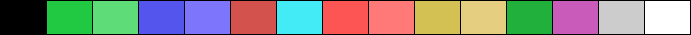
\includegraphics[scale=0.7]{TMS9918Apalette.png}

    \begin{itemize}
        \item VDP\_COLR\_TRNSP  - Transparent
        \item VDP\_COLR\_BLACK  - Black
        \item VDP\_COLR\_M\_GRN - Medium Green
        \item VDP\_COLR\_L\_GRN - Light Green
        \item VDP\_COLR\_D\_BLU - Dark Blue
        \item VDP\_COLR\_L\_BLU - Light Blue
        \item VDP\_COLR\_D\_RED - Dark Red
        \item VDP\_COLR\_CYAN   - Cyan
        \item VDP\_COLR\_M\_RED - Medium Red
        \item VDP\_COLR\_L\_RED - Light Red
        \item VDP\_COLR\_D\_YLW - Dark Yellow
        \item VDP\_COLR\_L\_YLW - Light Yellow
        \item VDP\_COLR\_D\_GRN - Dark Green
        \item VDP\_COLR\_MGNTA  - Magenta
        \item VDP\_COLR\_GREY   - Grey
        \item VDP\_COLR\_WHITE  - White
    \end{itemize}

    % ==========================================================================
    \subsection{Jiffy Counter}
    % ==========================================================================
    \label{subsec:jiffy_counter}

    A \textit{Jiffy} is the time between two ticks of the system timer interrupt.
    On the dastaZ80, this timer is generated by the TMS9918A (\textbf{VDP}) at
    roughly each 1/60th second.\\

    The counter is made of 3 bytes. Byte 1 is incremented in each \textbf{VDP}
    interrupt. Once it rolls over to zero (256 increments), the byte 2 is
    incremented. Once the byte 2 rolls over, the byte 3 is incremented. Once the
    three bytes together (24-bit) reach the value \texttt{0x4F1A00}, the three
    bytes are initialised to zero.

    \texttt{0x4F1A00} (5,184,000 in decimal) is the number of jiffies in 24
    hours: 24 hours x 60 minutes in an hour x 60 seconds in a minute x 60
    jiffies in a second.

    \textbf{IMPORTANT}: This counter MUST not be interpreted as an accurate
    clock, because when transferring data to the \textbf{VRAM} the OS disables
    the \hyperref[sec:nmi]{NMI}\footnote{It is also highly recommended that in
    your programs you also disable the \hyperref[sec:nmi]{NMI} when copying
    large amounts of data. Otherwise, the process will be interrupted 60 times
    per second, and therefore slow it down.}, and therefore the counter stops
    for a while.

    % ==========================================================================
    \subsection{OS Boot Sequence}
    % ==========================================================================
    After power on or after pressing the \textbf{RESET} button:

    \begin{itemize}
        \item \textbf{Bootstrap}
        \begin{itemize}
            \item Copy contents of the ROM into High RAM (\texttt{0x8000} - \texttt{0xFFFF}).
            \item Disable ROM chip and enable Low RAM (\texttt{0x0000} - \texttt{0x7FFF}).
            Therefore, all \textbf{MEMORY} is RAM from now on.
            \item Copy the copy of ROM inm High RAM to Low RAM. Bootstrap code is not copied.
            \item Transfer control to BIOS (\texttt{jp F\_BIOS\_SERIAL\_INIT}).
        \end{itemize}
        \item \textbf{Initialise SIO/2} (\texttt{F\_BIOS\_SERIAL\_INIT})
        \begin{itemize}
            \item Initialise SIO/2.
            \begin{itemize}
                \item Set Channel A as 115,000 bps, 8N1, Interrupt in all 
                received characters.
                \item Set Channel B as 115,000 bps, 8N1, Interrupt in all 
                received characters.
                \item Set Interrupt Vector to \texttt{0x60}.
            \end{itemize}
            \item Set CPU to Interrupt Mode 2.
            \item \texttt{jp F\_BIOS\_WBOOT}
        \end{itemize}
        \item \textbf{BIOS Boot} (\texttt{F\_BIOS\_WBOOT})
        \begin{itemize}
            \item Set SIO/2 Channel A as primary I/O.
            \item Transfer control to Kernel (\texttt{jp F\_KRN\_START}).
        \end{itemize}
        \item \textbf{Kernel Boot} (\texttt{F\_KRN\_START})
        \begin{itemize}
            \item Display dzOS welcome message.
            \item Display dzOS release version.
            \item Display Kernel version.
            \item Display available \textbf{RAM}.
            \item Initialise \textbf{VDP}.
            \begin{itemize}
                \item Test write/read \textbf{VRAM}.
                \item Set \textbf{Low Resolution Display} as \textit{Graphics II
                Bit-mapped Mode}.
                \item Show dastaZ80 Logo in the \textbf{Low Resolution Display}.
            \end{itemize}
            \item Initialise \textbf{FDD}.
            \item Initialise \textbf{SD Card}.
            \begin{itemize}
                \item Detect \textbf{SD Card}.
                \item Display number of available Disk Image Files.
                \item Display disk unit and name of each Disk Image File.
            \end{itemize}
            \item Initialise \textbf{Real-Time Clock (RTC)}.
            \begin{itemize}
                \item Detect \textbf{RTC}.
                \item Display current date and time.
                \item Display \textbf{RTC}'s battery status.
                \item Detect \textbf{NVRAM}.
            \end{itemize}
            \item Initialise \hyperref[sec:ram_memmap]{SYSVARS}.
            \begin{itemize}
                \item Set show deleted files with \textit{cat} command as OFF.
                \item Set default File Type as 0 (USR = User defined).
                \item Set default loadsave address to \texttt{0x0000} (i.e. will
                save/load starting from Free RAM (\texttt{0x4420})).
            \end{itemize}
            \item Set default \textbf{DISK} as 1 (i.e. first Disk Image File in
            the \textbf{SD card}).
            \item Transfer control to Command-line Interpreter (CLI) (\texttt{jp F\_CLI\_START}).
        \end{itemize}
        \item \textbf{CLI} (\texttt{F\_CLI\_START})
        \begin{itemize}
            \item Display CLI version.
            \item Clear command buffers
            \item Display prompt ($>$).
            \item Read command entered by user.
            \item Parse command.
            \item Execute corresponding subroutine.
            \item Loop back to Display prompt.
        \end{itemize}
    \end{itemize}

    % ==========================================================================
    \subsection{dzOS Programming Style}
    % ==========================================================================

    When writting dzOS and software for dzOS, the following style has been
    followed:

    \begin{itemize}
        \item All CPU registers are witten in uppercase (e.g. \textit{A},
        \textit{BC}, \textit{DE}, \textit{HL}).
        \item All CPU flags are witten in lowercase (e.g. \textit{z},
        \textit{nz}, \textit{c}, \textit{nc}, \textit{m}, \textit{p}).
        \item All assembly mnemonics are written in lowercase (e.g. 
        \textit{ld A,0}).
        \item Labels for subroutines that will be public (i.e. called via a
        Jumpblock) are written in uppercase.
        \item No mnemonics are written in the same line as a label.
        \item Public subroutines contain comments specifying:
        \begin{itemize}
            \item Short description.
            \item Input CPU registers or variables (SYSVARS).
            \item Output CPU registers or variables (SYSVARS).
        \end{itemize}
        \item All hexadecimal values are written with a dollar sign as prefix.
        \item Tabs are written as 4 spaces.
        \item Mnemonics start after 2 tabs (8 spaces).
        \item When possible, comments are written in column 41. Otherwise in
        next closest tab.
        \item Source code is heavily commented. Mostly on each line.
        \item \textit{The Telemark Assembler} (TASM) specific:
        \begin{itemize}
            \item \textit{.BYTE} is used instead of \textit{.DB}
            \item \textit{.WORD} is used instead of \textit{.DW}
        \end{itemize}
    \end{itemize}

    % ==========================================================================
    % Bibliography
    % ==========================================================================
    \pagebreak
    \bibliographystyle{unsrt}
    \bibliography{dastaZ80}
\end{document}